\pdfoutput=1

%\documentclass[preprint,10pt]{elsarticle}
\documentclass[preprint,10pt]{article}
%\documentclass[review]{siamart0216}
%\documentclass{siamart0216}

\usepackage{fullpage}
\usepackage{amsmath,amssymb,amsfonts,amsthm}
\theoremstyle{definition}
\newtheorem{definition}{Definition}
\theoremstyle{lemma}
\newtheorem{lemma}{Lemma}
\newtheorem*{remark}{Remark}
\theoremstyle{theorem}
\newtheorem{theorem}{Theorem}
\theoremstyle{assumption}
\newtheorem{assumption}{Assumption}
%\usepackage{thmtools}
%\declaretheorem[style=definition,qed=$\blacksquare$,numberwithin=chapter]{definition}

\usepackage[titletoc,toc,title]{appendix}

\usepackage{array} 
\usepackage{listings}
\usepackage{mathtools}
\usepackage{pdfpages}
\usepackage[textsize=footnotesize,color=green]{todonotes}
\usepackage{bm}
\usepackage{bbm}

%\usepackage{tikz}
\usepackage[normalem]{ulem}
\usepackage{hhline}

%% ====================================== alg package
\usepackage{algorithm}
\usepackage[noend]{algpseudocode}
\usepackage{algorithmicx}
\algblock{ParFor}{EndParFor}
% customising the new block
\algnewcommand\algorithmicparfor{\textbf{parfor}}
\algnewcommand\algorithmicpardo{\textbf{do}}
\algnewcommand\algorithmicendparfor{\textbf{end\ parfor}}
\algrenewtext{ParFor}[1]{\algorithmicparfor\ #1\ \algorithmicpardo}
\algrenewtext{EndParFor}{\algorithmicendparfor}
%% ====================================== end alg package

\usepackage{graphicx}
\usepackage{subfig}
\usepackage{color}

%% ====================================== graphics

\usepackage{pgfplots}
\usepackage{pgfplotstable}
\definecolor{markercolor}{RGB}{124.9, 255, 160.65}
\pgfplotsset{width=10cm,compat=1.3}
\pgfplotsset{
tick label style={font=\small},
label style={font=\small},
legend style={font=\small}
}

\usetikzlibrary{calc}

%%% START MACRO FOR ANNOTATION OF TRIANGLE WITH SLOPE %%%.
\newcommand{\logLogSlopeTriangle}[5]
{
    % #1. Relative offset in x direction.
    % #2. Width in x direction, so xA-xB.
    % #3. Relative offset in y direction.
    % #4. Slope d(y)/d(log10(x)).
    % #5. Plot options.

    \pgfplotsextra
    {
        \pgfkeysgetvalue{/pgfplots/xmin}{\xmin}
        \pgfkeysgetvalue{/pgfplots/xmax}{\xmax}
        \pgfkeysgetvalue{/pgfplots/ymin}{\ymin}
        \pgfkeysgetvalue{/pgfplots/ymax}{\ymax}

        % Calculate auxilliary quantities, in relative sense.
        \pgfmathsetmacro{\xArel}{#1}
        \pgfmathsetmacro{\yArel}{#3}
        \pgfmathsetmacro{\xBrel}{#1-#2}
        \pgfmathsetmacro{\yBrel}{\yArel}
        \pgfmathsetmacro{\xCrel}{\xArel}

        \pgfmathsetmacro{\lnxB}{\xmin*(1-(#1-#2))+\xmax*(#1-#2)} % in [xmin,xmax].
        \pgfmathsetmacro{\lnxA}{\xmin*(1-#1)+\xmax*#1} % in [xmin,xmax].
        \pgfmathsetmacro{\lnyA}{\ymin*(1-#3)+\ymax*#3} % in [ymin,ymax].
        \pgfmathsetmacro{\lnyC}{\lnyA+#4*(\lnxA-\lnxB)}
        \pgfmathsetmacro{\yCrel}{\lnyC-\ymin)/(\ymax-\ymin)} % THE IMPROVED EXPRESSION WITHOUT 'DIMENSION TOO LARGE' ERROR.

        % Define coordinates for \draw. MIND THE 'rel axis cs' as opposed to the 'axis cs'.
        \coordinate (A) at (rel axis cs:\xArel,\yArel);
        \coordinate (B) at (rel axis cs:\xBrel,\yBrel);
        \coordinate (C) at (rel axis cs:\xCrel,\yCrel);

        % Draw slope triangle.
        \draw[#5]   (A)-- node[pos=0.5,anchor=north] {}
                    (B)-- 
                    (C)-- node[pos=0.5,anchor=west] {#4}
                    cycle;
    }
}
%%% END MACRO FOR ANNOTATION OF TRIANGLE WITH SLOPE %%%.

\newcommand{\logLogSlopeTriangleNeg}[5]
{
    % #1. Relative offset in x direction.
    % #2. Width in x direction, so xA-xB.
    % #3. Relative offset in y direction.
    % #4. Slope d(y)/d(log10(x)).
    % #5. Plot options.

    \pgfplotsextra
    {
        \pgfkeysgetvalue{/pgfplots/xmin}{\xmin}
        \pgfkeysgetvalue{/pgfplots/xmax}{\xmax}
        \pgfkeysgetvalue{/pgfplots/ymin}{\ymin}
        \pgfkeysgetvalue{/pgfplots/ymax}{\ymax}

        % Calculate auxilliary quantities, in relative sense.
        \pgfmathsetmacro{\xArel}{#1}
        \pgfmathsetmacro{\yArel}{#3}
        \pgfmathsetmacro{\xBrel}{#1-#2}
        \pgfmathsetmacro{\yBrel}{\yArel}
        \pgfmathsetmacro{\xCrel}{\xArel}

        \pgfmathsetmacro{\lnxB}{\xmin*(1-(#1-#2))+\xmax*(#1-#2)} % in [xmin,xmax].
        \pgfmathsetmacro{\lnxA}{\xmin*(1-#1)+\xmax*#1} % in [xmin,xmax].
        \pgfmathsetmacro{\lnyA}{\ymin*(1-#3)+\ymax*#3} % in [ymin,ymax].
        \pgfmathsetmacro{\lnyC}{\lnyA+#4*(\lnxA-\lnxB)}
        \pgfmathsetmacro{\yCrel}{\lnyC-\ymin)/(\ymax-\ymin)} % THE IMPROVED EXPRESSION WITHOUT 'DIMENSION TOO LARGE' ERROR.

        % Define coordinates for \draw. MIND THE 'rel axis cs' as opposed to the 'axis cs'.
        \coordinate (A) at (rel axis cs:\xArel,\yArel);
        \coordinate (B) at (rel axis cs:\xBrel,\yBrel);
        \coordinate (C) at (rel axis cs:\xCrel,\yCrel);

        % Draw slope triangle.
        \draw[#5]   (A)-- node[pos=.5,anchor=south] {}
                    (B)-- 
                    (C)-- node[pos=0.5,anchor=west] {#4}
                    cycle;
    }
}
%%% END MACRO FOR ANNOTATION OF TRIANGLE WITH SLOPE %%%.

%%% START MACRO FOR ANNOTATION OF TRIANGLE WITH SLOPE %%%.
\newcommand{\logLogSlopeTriangleFlipNeg}[5]
{
    % #1. Relative offset in x direction.
    % #2. Width in x direction, so xA-xB.
    % #3. Relative offset in y direction.
    % #4. Slope d(y)/d(log10(x)).
    % #5. Plot options.

    \pgfplotsextra
    {
        \pgfkeysgetvalue{/pgfplots/xmin}{\xmin}
        \pgfkeysgetvalue{/pgfplots/xmax}{\xmax}
        \pgfkeysgetvalue{/pgfplots/ymin}{\ymin}
        \pgfkeysgetvalue{/pgfplots/ymax}{\ymax}

        % Calculate auxilliary quantities, in relative sense.
        %\pgfmathsetmacro{\xArel}{#1}
        %\pgfmathsetmacro{\yArel}{#3}
        \pgfmathsetmacro{\xBrel}{#1-#2}
        \pgfmathsetmacro{\yBrel}{#3}
        \pgfmathsetmacro{\xCrel}{#1}

        \pgfmathsetmacro{\lnxB}{\xmin*(1-(#1-#2))+\xmax*(#1-#2)} % in [xmin,xmax].
        \pgfmathsetmacro{\lnxA}{\xmin*(1-#1)+\xmax*#1} % in [xmin,xmax].
        \pgfmathsetmacro{\lnyA}{\ymin*(1-#3)+\ymax*#3} % in [ymin,ymax].
        \pgfmathsetmacro{\lnyC}{\lnyA+#4*(\lnxA-\lnxB)}
        \pgfmathsetmacro{\yCrel}{\lnyC-\ymin)/(\ymax-\ymin)} % THE IMPROVED EXPRESSION WITHOUT 'DIMENSION TOO LARGE' ERROR.

	\pgfmathsetmacro{\xArel}{\xBrel}
        \pgfmathsetmacro{\yArel}{\yCrel}

        % Define coordinates for \draw. MIND THE 'rel axis cs' as opposed to the 'axis cs'.
        \coordinate (A) at (rel axis cs:\xArel,\yArel);
        \coordinate (B) at (rel axis cs:\xBrel,\yBrel);
        \coordinate (C) at (rel axis cs:\xCrel,\yCrel);

        % Draw slope triangle.
        \draw[#5]   (A)-- node[pos=0.5,anchor=east] {#4}
                    (B)-- 
                    (C)-- node[pos=0.5,anchor=north] {1}
                    cycle;
    }
}
%%% END MACRO FOR ANNOTATION OF TRIANGLE WITH SLOPE %%%.


%%% START MACRO FOR ANNOTATION OF TRIANGLE WITH SLOPE %%%.
\newcommand{\logLogSlopeTriangleFlip}[5]
{
    % #1. Relative offset in x direction.
    % #2. Width in x direction, so xA-xB.
    % #3. Relative offset in y direction.
    % #4. Slope d(y)/d(log10(x)).
    % #5. Plot options.

    \pgfplotsextra
    {
        \pgfkeysgetvalue{/pgfplots/xmin}{\xmin}
        \pgfkeysgetvalue{/pgfplots/xmax}{\xmax}
        \pgfkeysgetvalue{/pgfplots/ymin}{\ymin}
        \pgfkeysgetvalue{/pgfplots/ymax}{\ymax}

        % Calculate auxilliary quantities, in relative sense.
        %\pgfmathsetmacro{\xArel}{#1}
        %\pgfmathsetmacro{\yArel}{#3}
        \pgfmathsetmacro{\xBrel}{#1-#2}
        \pgfmathsetmacro{\yBrel}{#3}
        \pgfmathsetmacro{\xCrel}{#1}

        \pgfmathsetmacro{\lnxB}{\xmin*(1-(#1-#2))+\xmax*(#1-#2)} % in [xmin,xmax].
        \pgfmathsetmacro{\lnxA}{\xmin*(1-#1)+\xmax*#1} % in [xmin,xmax].
        \pgfmathsetmacro{\lnyA}{\ymin*(1-#3)+\ymax*#3} % in [ymin,ymax].
        \pgfmathsetmacro{\lnyC}{\lnyA+#4*(\lnxA-\lnxB)}
        \pgfmathsetmacro{\yCrel}{\lnyC-\ymin)/(\ymax-\ymin)} % THE IMPROVED EXPRESSION WITHOUT 'DIMENSION TOO LARGE' ERROR.

	\pgfmathsetmacro{\xArel}{\xBrel}
        \pgfmathsetmacro{\yArel}{\yCrel}

        % Define coordinates for \draw. MIND THE 'rel axis cs' as opposed to the 'axis cs'.
        \coordinate (A) at (rel axis cs:\xArel,\yArel);
        \coordinate (B) at (rel axis cs:\xBrel,\yBrel);
        \coordinate (C) at (rel axis cs:\xCrel,\yCrel);

        % Draw slope triangle.
        \draw[#5]   (A)-- node[pos=0.5,anchor=east] {#4}
                    (B)-- 
                    (C)-- node[pos=0.5,anchor=south] {}
                    cycle;
    }
}
%%% END MACRO FOR ANNOTATION OF TRIANGLE WITH SLOPE %%%.



\usepackage{stmaryrd}


\renewcommand{\topfraction}{0.85}
\renewcommand{\textfraction}{0.1}
\renewcommand{\floatpagefraction}{0.75}

\newcommand{\vect}[1]{\ensuremath\boldsymbol{#1}}
\newcommand{\tensor}[1]{\underline{\bm{#1}}}
\newcommand{\del}{\triangle}
\newcommand{\curl}{\grad \times}
\renewcommand{\div}{\grad \cdot}

\newcommand{\bbm}[1]{\mathbbm{#1}}
\newcommand{\bs}[1]{\boldsymbol{#1}}
\newcommand{\equaldef}{\stackrel{\mathrm{def}}{=}}

\newcommand{\td}[2]{\frac{{\rm d}#1}{{\rm d}{\rm #2}}}
\newcommand{\pd}[2]{\frac{\partial#1}{\partial#2}}
\newcommand{\pdd}[2]{\frac{\partial^2#1}{\partial#2^2}}
\newcommand{\pdn}[3]{\frac{\partial^{#3}#1}{\partial#2^{#3}}}
\newcommand{\mb}[1]{\mathbf{#1}}
\newcommand{\mbb}[1]{\mathbb{#1}}
\newcommand{\mc}[1]{\mathcal{#1}}
\newcommand{\snor}[1]{\left| #1 \right|}
\newcommand{\nor}[1]{\left\| #1 \right\|}
\newcommand{\LRp}[1]{\left( #1 \right)}
\newcommand{\LRs}[1]{\left[ #1 \right]}
\newcommand{\LRa}[1]{\left\langle #1 \right\rangle}
\newcommand{\LRb}[1]{\left| #1 \right|}
\newcommand{\LRc}[1]{\left\{ #1 \right\}}
\newcommand{\LRceil}[1]{\left\lceil #1 \right\rceil}
\newcommand{\LRl}[1]{\left. #1 \right|}

%\newcommand{\cond}[1]{\kappa\LRp{#1}}
\newcommand{\cond}[2]{\nor{#1}_{#2}\nor{{#1}^{-1}}_{#2}}


\newcommand{\Grad} {\ensuremath{\nabla}}
\newcommand{\Div} {\ensuremath{\nabla\cdot}}
\newcommand{\jump}[1] {\ensuremath{\llbracket#1\rrbracket}}
\newcommand{\avg}[1] {\ensuremath{\LRc{\!\{#1\}\!}}}

\newcommand{\Oh}{{\Omega_h}}
\renewcommand{\L}{L^2\LRp{\Omega}}
\newcommand{\LK}{L^2\LRp{D^k}}
\newcommand{\LdK}{L^2\LRp{\partial D^k}}
\newcommand{\Dhat}{\widehat{D}}
\newcommand{\Lhat}{L^2\LRp{\Dhat}}

\newcommand{\eval}[2][\right]{\relax
  \ifx#1\right\relax \left.\fi#2#1\rvert}

\def\etal{{\it et al.~}}


\newcommand{\note}[1]{{\color{blue}{#1}}}


\newcommand{\LinfDk}{L^{\infty}\LRp{D^k}}

\newcommand{\diag}[1]{{\rm diag}\LRp{#1}}

\newcommand{\Ksub}{K_{\rm sub}}

\newcolumntype{C}[1]{>{\centering\let\newline\\\arraybackslash\hspace{0pt}}m{#1}}

%% d in integrand
\newcommand*\diff[1]{\mathop{}\!{\mathrm{d}#1}}


\makeatletter
\renewcommand\d[1]{\mspace{6mu}\mathrm{d}#1\@ifnextchar\d{\mspace{-3mu}}{}}
\makeatother

\date{}
\author{Jesse Chan}
\title{On discretely entropy conservative discontinuous Galerkin methods}

\begin{document}

\maketitle

\begin{abstract}
High order methods based on diagonal-norm summation by parts operators can be shown to semi-discretely conserve entropy for nonlinear systems of hyperbolic PDEs \cite{fisher2013high,carpenter2014entropy}.  These methods can be interpreted as mass lumped discontinuous Galerkin spectral element methods (DG-SEM) \cite{gassner2016split,gassner2016well,wintermeyer2017entropy, chen2017entropy}.  In this work, we describe how to extend discretely entropy conservative schemes for a more general class of DG methods using quadrature-based $L^2$ projections, flux differencing, and specific DG differentiation operators.  This approach also recovers existing methods for Burgers' equation involving generalized SBP operators without boundary nodes and dense norm SBP operators.  Numerical experiments confirm the stability and high order accuracy of the proposed methods for the one-dimensional shallow water and compressible Euler equations.  
\end{abstract}

%\tableofcontents

\section{Introduction}

Numerical simulations in engineering increasingly require higher accuracy without sacrificing computational efficiency.  High order methods are more accurate than low order methods per degree of freedom for sufficiently regular solutions, and provide one avenue towards improving fidelity in numerical simulations while maintaining reasonable computational costs.  High order methods which can accomodate unstructured meshes are particularly well-suited for problems with complex geometries.  Among such methods, high order discontinuous Galerkin (DG) methods are particularly well-suited to the solution of time-dependent hyperbolic problems on modern computing architectures \cite{hesthaven2007nodal, klockner2009nodal}.  

The accuracy observed for high order methods can be attributed in part to their low numerical dissipation and dispersion properties \cite{ainsworth2004dispersive}.  While low numerical dissipation is advantageous for problems in linear wave propagation \cite{chan2015gpu}, the high numerical dissipation present in low order schemes adds a stabilizing effect for nonlinear hyperbolic problems \cite{wang2013high}.  As a result, high order schemes for nonlinear conservation laws tend to require additional stabilization, including (but not limited to) filtering \cite{hesthaven2007nodal}, slope limiting \cite{krivodonova2007limiters}, artificial viscosity \cite{persson2006sub}, and polynomial de-aliasing \cite{ karniadakis2013spectral, kirby2003aliasing}.  Moreover, stabilized numerical methods can still fail, requiring user intervention or heuristic modifications to achieve non-divergent solutions.  

For linear wave propagation problems, numerical methods can be shown to be semi-discretely energy stable, even in the presence of curvilinear coordinates or variable coefficients \cite{warburton2013low, chan2016weight1, chan2016weight2, chan2017weight}.  This semi-discrete stability can be used to show that, under a stable timestep restriction (CFL), discrete solutions obtained by explicit time-stepping do not suffer from un-physical growth in time.  For nonlinear systems of conservation laws, typical methods for fluid dynamics do not admit formal proofs of stability.  However, progress has been made in designing provably discretely stable methods, beginning with the introduction of entropy conservative and entropy stable finite volume schemes by Tadmor \cite{tadmor1987numerical, tadmor2003entropy}.   These schemes rely on a specific entropy conservative flux which satisfies a condition involving the entropy variables and entropy potential, and have been extended to low order finite volume methods on unstructured grids \cite{ray2016entropy}.  

The construction of entropy conservative high order schemes was done much more recently for the compressible Euler and Navier-Stokes equations in \cite{fisher2013high, carpenter2014entropy} based on a spectral collocation approach on tensor product elements, which can be interpreted as a mass-lumped DG spectral element (DG-SEM) scheme.  The proof of entropy conservation relies on the presence of a diagonal mass matrix, as well as the summation by parts property \cite{gassner2013skew}.  Similar entropy-stable schemes were constructed for the shallow water and MHD equations \cite{gassner2016well, wintermeyer2017entropy,winters2017uniquely}.  More recently, entropy conservative and entropy stable schemes were extended to unstructured triangular meshes in \cite{chen2017entropy} using the split-form methodology of \cite{gassner2016split} and multi-dimensional SBP operators \cite{hicken2016multidimensional}.  

To the authors knowledge, the construction of entropy conservative and entropy stable schemes have relied on the use of lumped diagonal mass matrices and nodal collocation (diagonal norm SBP operators).  Entropy stable high order finite element and DG methods have been proposed \cite{hughes1986new}, but the proofs are often given at the continuous level, relying on exact integration or the chain rule, neither of which holds at the discrete level.  Thus, while DG-SEM based on flux differencing is entropy conservative, this is tied to a specific choice of basis and quadrature.  Diagonal-norm SBP operators can be constructed for triangles and tetrahedra \cite{chin1999higher,  hicken2016multidimensional, chen2017entropy}; however, the number of nodal points for such operators is greater than the dimension of the natural polynomial approximation space.  Furthermore, appropriate point sets have only been constructed for $N \leq 4$ in three dimensions \cite{zhebel2014comparison}.  
%Furthermore, diagonal-norm SBP operators do not naturally generalize to triangles or tetrahedra \cite{helenbrook2009existence}.  

This work focuses on the construction of entropy conservative high order DG schemes for systems of conservation laws.  In order to generalize beyond collocation DG and diagonal norm SBP operators, we will consider dense (non-lumped) mass matrices and more general quadrature rules (e.g.\ rules without boundary points, rules with more points than the dimension of the corresponding approximation space).  We will present proofs of discrete entropy stability in terms of integrals and $L^2$ projections, which we assume are computed using an appropriate quadrature rule.  We stress that, while we utilize a continuous notation involving integrals rather than discrete sums, the proofs rely only on properties of quadrature-based integration and $L^2$ projection.  

The outline of the paper is as follows: Section~\ref{sec:intro} will briefly review the construction of entropy conservative collocation methods on a single element.  Section~\ref{sec:ecdg} will describe how to construct analogous entropy conservative methods on single element.  Section~\ref{sec:ecdg2} will discuss extensions to multiple elements, including comparisons of different coupling terms and entropy stable fluxes.  We note that, for simplicity and clarity of presentation, the proposed methods and proofs are given in one dimension.  However, the extension to multiple dimensions (including simplicial elements) is straightforward and will be described in an upcoming manuscript.  
Finally, Section~\ref{sec:num} presents numerical results which verify the high order accuracy and discrete entropy conservation of the proposed methods.  


%\note{The construction of such operators on non-tensor product elements (such as simplices or pyramids) is non-trivial.} \cite{hicken2016multidimensional, chen2017entropy}.  \note{Constructing such operators for non-polynomial spaces (such as splines) is also difficult within the current framework.}


\section{Entropy conservative diagonal norm collocation DG methods}
\label{sec:intro}

We will begin by reviewing continuous entropy theory, as well as existing high order methods which are provably entropy conservative at the discrete level.  These methods were introduced in \cite{fisher2013high, carpenter2014entropy} for tensor product elements, though we adopt methods of proof introduced more recently in \cite{gassner2017br1, chen2017entropy}.  These methods all share a basis in diagonal norm summation by parts operators.  Because they can be derived from a nodal discontinuous Galerkin framework through the collocation of nodal points and quadrature points, we refer to them as ``diagonal norm collocation DG methods'' in this work.  

\subsection{Entropy stability for systems of hyperbolic PDEs}

%\note{Specify that all analysis is done in 1D but is extendable to higher dimensions!!  For simplicity and clarity of presentation, we will begin by focusing on the case $d = 1$.  }

We consider systems of nonlinear conservation laws in one dimension with $n$ variables
\begin{align}
%\pd{\bm{u}}{t} + \sum_{k=1}^d \pd{\bm{f_k(\bm{u})}}{x} &= 0, \qquad \bm{u}(x,t) = (u_1(x,t),\ldots,u_n(x,t)).
\pd{\bm{u}}{t} + \pd{\bm{f(\bm{u})}}{x} &= 0, \qquad \bm{u}(x,t) = (u_1(x,t),\ldots,u_n(x,t)).
\label{eq:pde}
\end{align}
where the fluxes $f(\bm{u})$ are smooth functions of the vector of conservative variables $\bm{u}({x},t)$.%$\bm{u}(x,t)$.
The Jacobian matrix $\bm{A}(\bm{u})$ is defined entrywise as
\[
%\LRp{\bm{A}_k(\bm{u})}_{ij} = \LRp{\pd{\bm{f}_k(\bm{u})}{\bm{u}_j}}_i.
\LRp{\bm{A}(\bm{u})}_{ij} = \LRp{\pd{\bm{f}(\bm{u})}{\bm{u}_j}}_i.
\]
We are interested in systems for which there exists a convex entropy function $U(\bm{u})$ such that  
\begin{equation}
%U''(\bm{u})\bm{A}_k(\bm{u}) = \LRp{U''(\bm{u}) \bm{A}_k(\bm{u})}^T.
U''(\bm{u})\bm{A}(\bm{u}) = \LRp{U''(\bm{u}) \bm{A}(\bm{u})}^T.
\label{eq:entropysym}
\end{equation}
For systems with convex entropy functions, one can define entropy variables $\bm{v} = U'(\bm{u})$.  The convexity of the $U(\bm{u})$ guarantees that the mapping between conservative and entropy variables is invertible.  

It can be shown (see, for example, \cite{mock1980systems}) that (\ref{eq:entropysym}) is equivalent to the existence of an entropy flux functions $F(\bm{u})$ such that
\[
\bm{v}^T \pd{\bm{f}}{\bm{u}} = \pd{F(\bm{u})}{\bm{u}}^T.
\]
The flux function and entropy flux function are further related through the so-called entropy potential $\psi_k$ 
\[
%\psi_k(\bm{v}) = \bm{v}^T\bm{f}_k(\bm{u}(\bm{v})) - F_k(\bm{u}(\bm{v})), \qquad \psi_k'(\bm{v}) = \bm{f}_k(\bm{u}(\bm{v})).
\psi(\bm{v}) = \bm{v}^T\bm{f}(\bm{u}(\bm{v})) - F(\bm{u}(\bm{v})), \qquad \psi'(\bm{v}) = \bm{f}(\bm{u}(\bm{v})).
\]

When $\bm{u}$ is smooth, multiplying (\ref{eq:pde}) on the left by $\bm{v}^T = U'(\bm{u})^T$, applying the definition of the entropy flux and using the chain rule yields the conservation of entropy
\[
\pd{U(\bm{u})}{t} + \pd{F(\bm{u})}{{x}} = 0.
\]
More generally, it can be shown that physically relevant solutions of (\ref{eq:pde}) (defined as the limiting solution for an appropriately defined vanishing viscosity) satisfy the entropy inequality
\[
\pd{U(\bm{u})}{t} + \pd{F(\bm{u})}{{x}} \leq 0.  
\]

We assume now that the domain is the interval $[-1,1]$.  Integrating the entropy inequality over this interval and using the definition of the entropy potential then yields
\begin{equation}
\int_{-1}^1 \pd{U(\bm{u})}{t} + \left.\LRp{\bm{v}^T\bm{f}(\bm{u}(\bm{v}))-\psi(\bm{v})}\right|_{-1}^1 \leq 0.  
\label{eq:consentropy}
\end{equation}
The focus of this work is the construction of methods which satisfy a discrete analogue of this entropy inequality.  We begin by reviewing existing discretely entropy conservative methods based on collocation and diagonal norm summation by parts (SBP) operators. 

\subsection{Entropy conservative collocation methods based on SBP operators}

Let ${x}_i \in [-1,1]$ denote the $(N+1)$ point Gauss-Lobatto-Legendre (GLL) quadrature rule with positive weights $w_1,\ldots,w_{N+1}$.  Let $\ell_i(x)$ denote the nodal Lagrange basis defined at GLL points, and define the differentiation matrix $\bm{D}$ be defined as 
\[
\bm{D}_{ij} = \pd{\ell_j(x_i)}{x}.
\]
The matrix $\bm{D}$ maps from nodal values of a polynomial to nodal values of its derivative.  We also define the mass matrix $\bm{M}$
\[
\bm{M}_{ij} = \int_{-1}^1 \ell_i(x)\ell_j(x)\diff{x} \approx \delta_{ij} w_i,
\]
where the approximation results from evaluating the integral using GLL quadrature.  For this choice of quadrature, the Kronecker property $\ell_j(x_i) = \delta_{ij}$ implies that $\bm{M}$ is a diagonal matrix whose entries are simply the quadrature weights.  

The mass and derivative matrices may be used to define the diagonal norm SBP operator $\bm{S} = \bm{M}\bm{D}$, with the summation-by-parts property 
\[
\bm{S} = \bm{B} - \bm{S}^T, \qquad \bm{B}_{ij} = \begin{cases}
1 &i = j = 1 \\
1 &i = j = N+1 \\
0 &\text{otherwise}
\end{cases}.
\]
This property is simply a restatement of integration by parts, using that the derivative of $\ell_j(x) \in P^{N-1}$ and that GLL quadrature is exact for polynomials of degree $2N-1$.  

We seek a polynomial approximation to the solution $\bm{u}(x)$ of (\ref{eq:pde}).  A DG formulation in the ``strong form'' \cite{hesthaven2007nodal} is given as
\[
\int_{-1}^1\LRp{ \pd{\bm{u}}{t} + \pd{\bm{f}(\bm{u})}{x}}\bm{w} + \left.\LRp{\bm{f}^* - \bm{f}(\bm{u})} \bm{w}\right|_{-1}^1 = 0, \qquad \forall \bm{w}\in V_h.
\]
Here, $\bm{f}^*$ is a numerical flux used for the weak imposition of boundary or continuity conditions.  

We derive a DG-SEM approximation by evaluating the above integrals using GLL quadrature.  We furthermore assume that the solution is approximated using a nodal basis at GLL points 
\[
\bm{u}(x,t) = \sum_{j=1}^{N+1} \bm{u}_j(t)\ell_j(x).  
\]
The resulting semi-discrete system yields a nodal collocation scheme for $\bm{u}_i$ 
\[
\pd{\bm{u}_i}{t} + \sum_{j=1}^{N+1}\LRp{\LRp{\bm{D}\otimes \bm{I}}_{ij}\bm{f}(\bm{u}_j) +\LRp{\bm{M}^{-1}\bm{B}}_{ij}(\bm{f}_i^* - \bm{f}(\bm{u}_i))} = 0.
\]

This formulation conserves the quantities $\bm{u}_i$, but (except in specific cases) does not satisfy a discrete analogue of the statement of entropy conservation (\ref{eq:consentropy}).  Entropy conservative schemes may be constructed based on the SBP property and a ``flux differencing'' approach \cite{gassner2016split} involving a definition of entropy conservative/stable fluxes given by Tadmor \cite{tadmor1987numerical, tadmor2003entropy}.  
\begin{definition}
Let $\bm{f}_S(\bm{u}_L,\bm{u}_R)$ be a bivariate function such that it is symmetric and consistent with the flux function $\bm{f}(\bm{u})$
\[
\bm{f}_S(\bm{u}_L,\bm{u}_R) = \bm{f}_S(\bm{u}_R,\bm{u}_L), \qquad \bm{f}_S(\bm{u},\bm{u}) = \bm{f}(\bm{u})
\]
The numerical flux $\bm{f}_S(\bm{u}_L, \bm{u}_R)$ is entropy conservative if, for entropy variables $\bm{v}_L = \bm{v}(\bm{u}_L), \bm{v}_R = \bm{v}(\bm{u}_R)$
\[
\LRp{\bm{v}_L - \bm{v}_R}^T \bm{f}_S(\bm{u}_L,\bm{u}_R) = (\psi_L - \psi_R), \qquad \psi_L = \psi(\bm{v}(\bm{u}_L)), \quad \psi_R = \psi(\bm{v}(\bm{u}_R)).  
\]
Similarly, a flux $\bm{f}_S(\bm{u}_L, \bm{u}_R)$ is referred to as entropy stable if $\LRp{\bm{v}_L - \bm{v}_R}^T \bm{f}_S(\bm{u}_L,\bm{u}_R) \leq (\psi_L - \psi_R)$.
\label{def:tadmor}
\end{definition}
An entropy conservative nodal collocation method can then be derived by modifying the flux derivative as follows
\begin{equation}
\pd{\bm{u}_i}{t} + \sum_{j=1}^{N+1}\LRp{\LRp{2\bm{D}\otimes \bm{I}}_{ij}\bm{f}_S(\bm{u}_i,\bm{u}_j) +\LRp{\bm{M}^{-1}\bm{B}}_{ij}(\bm{f}_i^* - \bm{f}(\bm{u}_i))}= 0.
\label{eq:dgsem}
\end{equation}
The replacement of the derivative of the flux function with flux differencing allows one to prove that (\ref{eq:dgsem}) conserves a discrete entropy \cite{gassner2017br1,chen2017entropy}.  We reproduce these proofs here, as we will refer to them in following sections.  
\begin{theorem}
The collocation method (\ref{eq:dgsem}) is discretely entropy conservative in the sense that
\[
\bm{1}^T\LRp{\bm{M}\pd{U(\bm{u})}{t} + \bm{B}\LRp{\bm{v}^T\bm{f}^* - \bm{\psi}}} = 0,
\]
where $\bm{1}$ denotes the vector of ones and $\bm{\psi}_i = \psi(\bm{v}_i)$ is the entropy potential in terms of the nodal value of $\bm{u}_i$.  
\label{thm:dgsem}
\end{theorem}
\begin{proof}
Let $\bm{v}_i = \bm{v}(\bm{u}_i)$ denote the entropy variables, defined in terms of the nodal values $\bm{u}_i$.  We multiply (\ref{eq:dgsem}) by $\LRp{\bm{M}\bm{v}}^T$.  
Using the fact that $\bm{M}$ is diagonal, the time derivative term can be manipulated to 
\[
\bm{v}^T\bm{M}\pd{\bm{u}}{t} = \sum_{i=1}^{N+1} \bm{M}_{ii} \bm{v}_i^T \pd{\bm{u}_i}{t} = \sum_{i=1}^{N+1} \bm{M}_{ii} \pd{S_i}{t} = \bm{1}^T\bm{M}\pd{S_i}{t},
\]
where we have used continuity in time to arrive at the point-wise relation 
\[
\bm{v}^T \pd{\bm{u}}{t} = \pd{U(\bm{u})}{\bm{u}}^T \pd{\bm{u}}{t} = \pd{U(\bm{u})}{t}.
\]

The spatial derivative term can be manipulated using the summation by parts property $\bm{M}\bm{D} = \bm{S} = \bm{B}-\bm{S}^T$
\begin{align}
\sum_{i,j=1}^{N+1} \bm{v}_i^T 2 \bm{M}\bm{D}_{ij}\bm{f}_S(\bm{u}_i,\bm{u}_j) &= \sum_{i,j=1}^{N+1} \bm{v}_i^T (\bm{S} + \bm{B} - \bm{S}^T)_{ij}\bm{f}_S(\bm{u}_i,\bm{u}_j) \nonumber\\
&= \sum_{i,j=1}^{N+1} \bm{S}_{ij}\bm{v}_i^T \bm{f}_S(\bm{u}_i,\bm{u}_j) - \bm{S}_{ji}\bm{v}_i^T \bm{f}_S(\bm{u}_i,\bm{u}_j) + \bm{B}_{ij}\bm{v}_i^T \bm{f}_S(\bm{u}_i,\bm{u}_j). \label{eq:sbpentropy}
\end{align}
Rearranging indices and using symmetry of $\bm{f}_S(\bm{u}_i,\bm{u}_j)$ then yields that
\begin{align*}
\sum_{i,j=1}^{N+1} \bm{S}_{ij}\bm{v}_i^T \bm{f}_S(\bm{u}_i,\bm{u}_j) - \bm{S}_{ji}\bm{v}_i^T \bm{f}_S(\bm{u}_i,\bm{u}_j) &= \sum_{i,j=1}^{N+1} \bm{S}_{ij} \LRp{\bm{v}_i - \bm{v}_j}^T\bm{f}_S(\bm{u}_i,\bm{u}_j)\\
&= \sum_{i,j=1}^{N+1} \bm{S}_{ij} \LRp{\bm{\psi}_i-\bm{\psi}_j} = -\bm{1}^T \bm{S}\bm{\psi} = -\bm{1}^T\bm{B}\bm{\psi},
\end{align*}
where we have used $\bm{S}\bm{1} = 0$ and the summation by parts property in the last line.  

Using that $\bm{B}$ is diagonal, combining the latter term in (\ref{eq:sbpentropy}) with boundary terms involving the numerical flux yields
\[
\sum_{i,j = 1}^{N+1} \bm{B}_{ij}\bm{v}_i^T \bm{f}_S(\bm{u}_i,\bm{u}_j) + \bm{v}_i^T\bm{B}_{ij}\LRp{\bm{f}_i^* - \bm{f}(\bm{u}_i)} = \bm{1}^T\bm{B} \LRp{\bm{v}^T \bm{f}^*},
\]
where we have used the consistency of $\bm{f}_S(\bm{u},\bm{u}) = \bm{f}(\bm{u})$.  Combining everything results in a discrete statement of the conservation of entropy (\ref{eq:consentropy}).   
%Combining everything results in a discrete statement of the conservation of entropy (\ref{eq:consentropy}) 
%\[
%\bm{1}^T\LRp{\bm{M}\pd{U(\bm{u})}{t} + \bm{B}\LRp{\bm{v}^T\bm{f}^* - \bm{\psi}}} = 0.
%\]
\end{proof}
We note that, unlike the proof of continuous entropy conservation, the proof of discrete entropy conservation does not require the use of the chain rule, which may not hold at the discrete level.  This proof of entropy conservation can also be extended beyond a single element by specifying appropriate simultaneous approximation terms (SBP-SAT).  This can be done by taking $\bm{f}_i^*$ to be the entropy conservative flux $f_S(u_L,u_R)$ at the interface between two elements \cite{carpenter2014entropy, gassner2017br1, chen2017entropy}.  Similarly, employing an entropy stable flux at element interfaces results in an entropy stable method which satisfies a global entropy inequality.  

It is important to emphasize that conservation of entropy does not, in general, guarantee stability of the numerical scheme unless the solution satisfies additional constraints.  For example, the convex entropy associated with the compressible Euler and Navier-Stokes equations is well-defined only if the density and pressure are positive, and steps must be taken in any numerical scheme to guarantee that the discrete solution of such constraints.  For DG methods, this is most commonly done using bound and positivity-preserving limiters, such as those introduced in \cite{zhang2010positivity, zhang2012maximum}.  



\section{Entropy conservative DG methods on a single element}
\label{sec:ecdg}

In this section, we focus on constructing entropy conservative DG schemes for general choices of basis and quadrature.  These include (as special cases) dense norm SBP operators and generalized SBP (GSBP) operators which do not contain boundary points, which introduce additional difficulties in constructing entropy conservative DG schemes.  These difficulties present themselves primarily in two areas: 
\begin{enumerate}
\item the generalization of flux differencing to a continuous formulation.  
\item the proof of entropy stability assumes a diagonal norm mass matrix, which commutes with point-wise multiplication by the (nodal values of) the entropy variables.  
\end{enumerate}

We address both areas of difficulty in generalizing the entropy conservative DG-SEM scheme (\ref{eq:dgsem}).  In particular, we give a continuous DG formulation with flux differencing, and prove that the generalized scheme is entropy conservative (stable) on a single element in the following sections.  As an example, we illustrate how to apply the proposed methods to produce energy conservative formulations of Burgers' equation.  

% to a larger class of quadratures and choices of basis.  Additionally, we prove that the generalized scheme is entropy conservative (stable) on multiple elements in the following sections.  

%We will get around these difficulties for dense-norm DG methods by satisfying three requirements for entropy stability
%\begin{itemize}
%\item $\bm{D}\bm{1} = 0$ for use of the flux formulation.  
%\item For some norm matrix $\bm{W}$, $\bm{W}\bm{D} = \bm{B}-\bm{D}^T\bm{W}$ where $\bm{B}$ is a suitably defined boundary operator.
%\item Contraction with the \textit{projection} of the entropy variables.  
%\end{itemize}

\subsection{Notation}

\note{Fix notation: switch $V_h$ to $P^N$}
We assume that the domain $\Omega \in \mathbb{R}^d$ is exactly triangulated by a mesh which consists of the union of non-overlapping elements $D^k$.  We further assume that each element $D^k$ is the image of a reference element $\widehat{D}$ under the local elemental mapping 
\[
x^k = \bm{\Phi}^k \widehat{x},
\]
where $x^k$ denote physical coordinates on $D^k$ and $\widehat{x}$ denote coordinates on the reference element.  Finally, we identify $J$ as the determinant of the Jacobian of $\bm{\Phi}^k$, and refer to it as the Jacobian for the remainder of this work.  For clarity and simplicity of presentation, we assume $\bm{\Phi}^k$ is affine in this case, such that $J$ is constant over each element $D^k$.  

We will approximate solution components over each element $D^k$ from an approximation space $V_h\LRp{D^k}$, which we define as the composition of the mapping $\bm{\Phi}^k$ and a reference approximation space $V_h\LRp{\widehat{D}}$
\[
V_h\LRp{D^k} = \bm{\Phi}^k \circ V_h\LRp{\widehat{D}}.
\]
The global approximation space $V_h\LRp{\Omega}$ is then defined as the direct sum of local approximation spaces
\[
V_h\LRp{\Omega} = \bigoplus_{D^k}V_h\LRp{D^k}.  
\]
We assume that $V_h(D^k) \subset H^1(D^k)$; in other words, that all elements of each local approximation space are square integrable and admit well-defined traces.  

We define the $L^2$ norm and inner products over the element $D^k$ and the surface of the element $\partial D^k$\footnote{In one dimension, $D^k$ is some interval $[x_L,x_R]$ and the $L^2$ inner product over the surface reduces to 
\[
\LRa{u,v}_{\partial D^k} = u(x_L)v(x_L) + u(x_R)v(x_R).
\]
However, the presented proofs in this work will not utilize this simplification, and are thus generalizable to higher dimensions in a straightforward manner.}
\[
\LRp{u,v}_{D^k} = \int_{D^k} u v\diff{x}, \qquad \nor{u}^2_{D^k} = (u,u)_{D^k}, \qquad \LRa{u,v}_{\partial D^k} = \int_{\partial D^k} u v \diff{x}.
\]
We also define the local $L^2$ projection operator $\Pi_N: L^2(D^k)\rightarrow V_h(D^k)$ such that
\[
\LRp{\Pi_N u,v}_{D^k} = \LRp{u,v}_{D^k}, \qquad \forall v\in V_h\LRp{D^k}.  
\]
Throughout this work, we will use that this definition of the $L^2$ projection holds even when integrals are approximated using quadrature.  We will make no assumptions on quadrature except that \note{specify assumptions - integrate polynomials of degree $N$ on the reference element exactly, such that integration by parts holds.  Add footnote that we can also generalize to the under-integrated case.  }


Finally, we define the jump and average of discontinuous functions across element interfaces.  Let $D^{k,+}$ denote the neighboring element of across a face $f$ of $D^k$, and let $u^+$ denote the values of $u$ on $D^{k,+}$.  The jump of $u$ across $f$ on $D^k$ is then defined as
\[
\jump{u} = u^+ - u, \qquad \avg{u} = \frac{u^+ + u}{2}.
\]
The jump and average of vector fields are defined component-wise using the jumps and averages of components.  When the face $f$ lies on the boundary, we define $u^+ = u$, such that $\jump{u} = 0$ and $\avg{u} = u$ on $\partial \Omega$.


\subsection{A continuous interpretation of flux differencing}

In this section, we offer a continuous interpretation of flux differencing \cite{fisher2013high,gassner2017br1,chen2017entropy}, which also encompasses the split form methodology proposed in \cite{gassner2016split}.  This interpretation will guide the construction of entropy conservative DG schemes.  

Assume that $\bm{f}_S(\bm{u}_L,\bm{u}_R)$ is the symmetric and consistent two-point flux defined in (\ref{def:tadmor}).  Consider the bilinear function
\[
\bm{f}_S\LRp{\bm{u}(x),\bm{u}(y)}, \qquad x, y \in \mathbb{R}.  
\]
Flux differencing can be interpreted as differentiating $\bm{f}_S\LRp{\bm{u}(x),\bm{u}(y)}$ along one coordinate $x$, then evaluating the result with $y=x$
\begin{equation}
\pd{\bm{f}(\bm{u}(x))}{x} \Longrightarrow 2\left.\pd{\bm{f}_S\LRp{\bm{u}(x),\bm{u}(y)}}{x}\right|_{y=x}.
\label{eq:fluxdiff}
\end{equation}
It was shown in \cite{chen2017entropy} that flux differencing is a consistent approximation of the flux derivative.  
%Since the two-point flux is consistent, 

%\subsubsection{Illustration using Burgers' equation}

It is helpful to first understand flux differencing as a method for recovering split formulations.  We illustrate this using the one-dimensional Burgers equation on domain $ [-1,1]$, which is given in conservative form as 
\[
\pd{u}{t} + \pd{f(u)}{x} = 0, \qquad f(u) = \frac{1}{2}u^2.
\]
%An alternative form of the Burgers' equation can be derived by taking a convex combination of the conservative and non-conservative forms of the spatial term
%\begin{equation}
%\pd{u}{t} + \frac{1}{3}\LRp{\pd{u^2}{x} + u\pd{u}{x}} = 0.
%\label{eq:burgerssplit}
%\end{equation}
Assuming smooth $u$, Burgers' equation conserves a square entropy $U(\bm{u}) = u^2/2$.   This can be shown by multiplying by $u$, integrating over $[-1,1]$, and using $\pd{u}{t}u = \frac{1}{2}\pd{u^2}{t}$
\begin{equation}
\frac{1}{2}\pd{}{t}\int_{-1}^1{u}^2 = -\left.\frac{u^3}{3}\right|_{-1}^1.
\label{eq:burgersconservation}
\end{equation}

It is well known that DG formulations based on a split formulation can be shown to conserve the square entropy $u^2$ \cite{gassner2013skew, ranocha2017extended}.  This form may be also be recovered using flux differencing under the two-point flux
\[
f_S(u_L,u_R) = \frac{1}{6}(u_L^2 + u_Lu_R + u_R^2).
\]
Applying (\ref{eq:fluxdiff}) yields the split form of Burgers' equation
\[
2\left.\pd{f_S(u(x),u(y))}{x}\right|_{y=x} = \frac{1}{3}\left.\pd{\LRp{u(x)^2 + u(x)u(y) + u(y)^2}}{x}\right|_{y=x} = \frac{1}{3}\LRp{\pd{u^2}{x} + u\pd{u}{x}}.
\]
We note that recovering the split-form of Burgers' equation relies on the property
%\footnote{This is also the reason why the factor of $2$ is necessary when using flux differentiation (\ref{eq:fluxdiff}); the differentiation of terms which depend only on $y$ vanish, \note{finish...}.}
that 
\[
\pd{\LRp{u(y)^2}}{x} = u(y)^2\pd{\LRp{1}}{x} = 0.  
\]
Thus, recovery of the split form can be achieved by using flux differencing in combination with any differential operator $D$ such that $D1 = 0$.  
%\[
%D:L^2 \rightarrow V_h, \qquad D1 = 0.
%\]
%For Burgers' equation (as well as any skew-symmetric splitting), replacing the exact derivative $\pd{}{x}$ by $D$ will again recover a statement of the split formulation (\ref{eq:burgerssplit}) 
%\[
%\pd{u}{t} + \frac{1}{3}\LRp{Du^2 + uDu} = 0.
%\]
%The introduction of $D$ is necessary when adapting the flux differentiation procedure in the context of numerical discretizations.  

\subsection{Discrete differential operators and weighted integration by parts}

Both the conservative and split forms of Burgers' equation are equivalent at the continuous level (assuming continuity of $u$ and exact differentiation); however, this is no longer true at the discrete level.  Suppose now that the solution is approximated by $u \in V_h(\Omega)$ on a single element.  Since $f(u) = u^2/2 \not\in V_h(\Omega)$ for general choices of $u, V_h$, it is not possible to differentiate $f(u)$ exactly without prior knowledge of the form of the nonlinearity.  Indeed, it is more common to first project $f(u)$ to $V_h$, then differentiate, such that the discrete scheme is equivalent to solving for $u \in V_h(\Omega)$ such that
\[
\int_{-1}^1 \LRp{\pd{u}{t} + \pd{\Pi_N f(u)}{x}}w \diff{x}  
%\int_{-1}^1 \LRp{\pd{u}{t} +D_N f(u)}w \diff{x} 
=0, \qquad \forall w \in V_h(\Omega).  
\]
This scheme does not, in general, conserve energy.  %Moreover, if $\Pi_N$ is computed using quadrature, rewriting the scheme into this form suggests that de-aliasing techniques based on over-integration hit a ``bottleneck'', due to the fact that increasing quadrature accuracy only increases the accuracy of the projection \cite{kirby2003aliasing}.  

We can derive a semi-discrete Galerkin scheme based which conserves energy discretely using flux differencing and a different choice of discrete differentiation operator $D_N$, which was motivated by the SBP operators introduced in \cite{chen2017entropy}.  Let $w(x)$ be some bounded real-valued function; then, we can define the discrete differential operator $D_N: H^1\rightarrow V_h$ such that, for $u\in H^1$, 
\begin{align}
\LRp{D_N u, vw}_{\widehat{D}} = \LRp{\pd{ \Pi_N u}{x},vw}_{\widehat{D}} + \frac{1}{2}{\LRa{{u - \Pi_N u}, vw\bm{n}_x}}_{\partial \widehat{D}} + \frac{1}{2}\LRa{u - \Pi_Nu ,\Pi_N\LRp{vw}\bm{n}_x }_{\widehat{D}}, \qquad \forall v\in V_h.
\label{eq:dgd}
\end{align}
This operator satisfies a form of integration by parts, which is summarized by the following lemma:
\begin{lemma}
\label{lemma:dgd_local}
The linear operator $D_N$ satisfies a ``weighted'' integration by parts property with respect the $L^2$ inner product and any bounded real-valued function $w(x)$ 
\[
\LRp{D_N u, wv}_{\widehat{D}} = \LRa{u,wv\bm{n}_x}_{\partial \widehat{D}} - \LRp{u,D_N (w v)}_{\widehat{D}}.
\]
\end{lemma}
\begin{proof}
Integrating the left hand side by parts gives
\[
-\LRp{\pd{ \Pi_N (vw)}{x},u}_{\widehat{D}} + \frac{1}{2}{\LRa{{u - \Pi_N u}, vw\bm{n}_x}}_{\partial \widehat{D}} + \frac{1}{2}\LRa{u + \Pi_Nu ,\Pi_N\LRp{vw}\bm{n}_x }_{\partial \widehat{D}}, \qquad \forall v\in V_h.
\]
Rearranging boundary terms yields
\[
-\LRp{\pd{ \Pi_N (vw)}{x},u}_{\widehat{D}} + \frac{1}{2}\LRa{vw + \Pi_N(vw) , u\bm{n}_x }_{\partial \widehat{D}}  - \frac{1}{2}\LRa{vw - \Pi_N (vw), \Pi_N u \bm{n}_x}_{\partial \widehat{D}}.  
\]
Adding and subtracting $\LRa{vw,u\bm{n}_x}_{\partial \widehat{D}}$ completes the proof.
\end{proof}

Direct computations also show that $\LRp{D_N 1,vw}_{\widehat{D}} = 0$ for all bounded weights $w(x)$ and $\forall v \in V_h$.  Thus, we can apply (\ref{eq:fluxdiff}) with $D_N$ to construct a discrete formulation for Burgers' equation
\begin{align}
\LRp{\pd{u}{t},v} + \frac{1}{3}\LRp{D_N u^2 + uD_Nu,v} &= \LRp{\pd{u}{t},v}_{\widehat{D}} + \frac{1}{3}\LRp{D_N u^2,v}_{\widehat{D}} + \frac{1}{3}\LRp{D_Nu,uv}_{\widehat{D}},
%\LRp{\pd{u}{t},v}_{\widehat{D}} + \frac{1}{3}\LRp{\pd{\Pi_N u^2}{x},v}_{\widehat{D}} + \frac{1}{3}\LRp{D_Nu,uv}_{\widehat{D}}
\qquad \forall v\in V_h.
\label{eq:burgersdiscrete}
\end{align}
To show this formulation is discretely energy conservative, we take $v=u$ and use Lemma~\ref{lemma:dgd_local} to cancel volume terms, yielding
\[
\frac{1}{2}\pd{}{t}\LRp{u,u}_{\widehat{D}} = -\frac{1}{3}\LRa{u^2,u}_{\partial \widehat{D}},
\]
which is a discrete analogue of the conservation condition (\ref{eq:burgersconservation}).  This is equivalent to the skew-symmetric split formulation described in \cite{gassner2013skew}; however, as noted in \cite{chen2017entropy}, it can be derived from flux differencing without explicit knowledge of the skew form.  We will show later in Section~\ref{sec:recovery} that a natural extension of this formulation to multiple elements recovers the weak form of the scheme introduced in \cite{ranocha2017extended}.  

%We note that the $L^2$ projection appears within the boundary terms.  While this may not pose a significant problem on one element, in the case of multiple elements, it introduces an all-to-all coupling between degrees of freedom on elements which share a face \cite{fernandez2016simultaneous}.  In the following section, we describe an alternative choice of discrete differential operator $D$ inspired by Chen and Shu \cite{chen2017entropy} which avoids this problem of increased bandwidth while maintaining properties which are necessary to guarantee provably discrete entropy conservation.  

%Using the fact integration by parts holds when considering two elements of $V_h$, and that $\LRp{\Pi_N u^2, v} = \LRp{u^2,v}$ for any $v \in V_h$, it can be shown that the volume terms cancel out for $v = u$, leaving only boundary terms (which is a prerequisite of energy/entropy stability).  

\subsection{Conservation of entropy on one element}

While flux differencing can be used to recover split formulations, it can also be used to construct entropy stable formulations which do not correspond to skew-symmetric splittings.  In this section we will show that, for any sufficiently accurate quadrature rule, it is possible to construct discretizations which satisfy a discrete equivalent of conservation of entropy (\ref{eq:consentropy}).  

For the proof, we will need the following assumption:
\begin{assumption}
The numerical flux function $\bm{f}_S$ admits an absolutely convergent expansion of the form 
\[
\bm{f}_S(x,y) = \sum_{i=1}^{\infty} \bm{f}_i(x) \bm{g}_i(y), 
\]
where $\bm{f}_i, \bm{g}_i$ are real and bounded over each element $D^k$.  
\label{eq:assumption}
\end{assumption}
This assumption is satisfied, for example, by $\bm{f}_S$ which are real analytic and thus admit a Taylor expansion in $x$ and $y$.  In Appendix~\ref{appendix:A}, we show that this assumption also holds for the choices of flux functions $\bm{f}_S$ considered in this work, assuming the solution satisfies physical bound constraints.  However, we note that this assumption is not required in the computation implementations of the proposed methods, and may be an overly restrictive condition on $\bm{f}_S$.  

We now introduce a discretization for the nonlinear system of conservation laws (\ref{eq:pde}) on $[-1,1]$: find $\bm{u}\in V_h$ such that
\begin{equation}
\LRp{\pd{\bm{u}}{t},\bm{w}}_{\widehat{D}} + \LRp{\left.\LRp{2D_N \bm{f}_S(\bm{u}_{\bm{v}}(x),\bm{u}_{\bm{v}}(y))}\right|_{y=x},\bm{w}}_{\widehat{D}}= \LRa{\bm{f}^*-\bm{f}(\bm{u}_{\bm{v}}),\bm{w}}_{\partial \widehat{D}}, \qquad \bm{w}\in V_h,
\label{eq:ecdg_oneelem}
\end{equation}
where $\bm{f}^*$ is a numerical flux used to impose boundary conditions weakly, and $\bm{u}_{\bm{v}}(x),\bm{u}_{\bm{v}}(y)$ are evaluations of $\bm{u}$ in terms of the projections of entropy variables $\bm{v}(\bm{u}(x))$ 
\begin{equation}
%\bm{u}_{\bm{v}}(x) = \bm{u}(\Pi_N\bm{v}(\bm{u}(x))), \qquad \bm{u}_{\bm{v}}(y) = \bm{u}(\Pi_N\bm{v}(\bm{u}(y))).
\bm{u}_{\bm{v}}(x) = \bm{u}\LRp{(\Pi_N\bm{v})(x)}.
\label{eq:projectedentropyvars}
\end{equation}

%We first introduce matrices defined over $[-1,1]$.  We assume some discrete quadrature rule on the reference element consisting of $N_q$ points ${\bm{x}}_q = \LRc{{x}_1,\ldots,{x}_{N_q}}$ and quadrature weights $\bm{w}_q = \LRc{w_1,\ldots,w_{N_q}}$.  Let $\bm{W}$ denote the diagonal matrix whose entries are quadrature weights. Then, assuming that each component of $\bm{u}$ is represented in some basis $\phi_j(x)$ of dimension $N_p$ which spans $V_h$
%\[
%V_h = {\rm span}\LRc{\phi_j(\widehat{x})}_{j=1}^{N_p},
%\]
%we can define the quadrature interpolation matrix $\bm{V}_q$
%\[
%\LRp{\bm{V}_q}_{ij} = \phi_j(\widehat{x}_i), \qquad 1 \leq j \leq N_p, \qquad 1 \leq i \leq N_q.  
%\]
%Given $\bm{V}_q$, we introduce the mass matrix $\bm{M} = \bm{V}_q^T\bm{W}\bm{V}_q$, as well as the quadrature-based $L^2$ projection operator $\bm{P}_q$
%\[
%\bm{P}_q = \bm{M}^{-1}\bm{V}_q^T\bm{W}.
%\]
%Let $\bm{D}_x$ denote the differentiation matrix defined implicitly through
%\[
%u(x) = \sum_{j=1}^{N_p}\bm{u} \phi_j(\widehat{x}), \qquad \pd{u}{\widehat{x}} = \sum_{j=1}^{N_p} \LRp{\bm{D}_x \bm{u}}_j\phi_j(\widehat{x})
%\]
%In other words, $\bm{D}_x$ maps basis coefficients of some function $u \in V_h$ to coefficients of its derivative on $[-1,1]$.  
%
%Finally, we introduce matrices used to compute boundary terms.  Let $\bm{V}_f$ denote the matrix which interpolates to boundary values\footnote{In generalizing to higher dimensions, $\bm{V}_f$ would be the matrix which interpolates to surface quadrature points.}
%\[
%\LRp{\bm{V}_f}_{1j} = \phi_j(-1), \qquad \LRp{\bm{V}_f}_{2j} = \phi_j(1), \qquad 1 \leq j \leq N_p.  
%\]
%Furthermore, let $\bm{W}_f$ denote the diagonal matrix of surface quadrature weights, which is simply the $2\times 2$ identity matrix in one dimension.  
%
%Together, these matrices can be used to define the quadrature-based differentiation matrix $\bm{D}_q$
%\[
%\bm{D}_q = \bm{V}_q \bm{D}_x \bm{P}_q,
%\]
%which is a discrete analogue to $D_N$.  It is straightforward then to show that this matrix satisfies properties similar to summation-by-parts:
%\begin{lemma}
%Let $\bm{n}_x = [-1,1]$ be the vector of unit normals in one dimension.  Then, 
%\[
%\bm{W}\bm{D}_q = \bm{P}_q^T\bm{V}_f^T\bm{W}_f {\rm diag}(\bm{n}_x) \bm{V}_f \bm{P}_q  - \bm{D}_q^T \bm{W}, \qquad \bm{1}^T\bm{W}\bm{D}_q =  \bm{1}^T\bm{W}_f {\rm diag}(\bm{n}_x) \bm{V}_f \bm{P}_q.  
%\]
%\label{lemma:sbp}
%\end{lemma}
%\begin{proof}
%\note{Finish}
%\end{proof}


%Let $\bm{u}^k$ now denote the vector of coefficients for the $k$th component of $\bm{u}(x)$.  The formulation (\ref{eq:ecdg_oneelem}) is equivalent to the semi-discrete system:
%\begin{equation}
%\bm{M} \td{\bm{u}^k}{t} + \bm{V}_q^T\bm{W}{\rm diag}\LRp{\bm{V}_q\bm{D}_x\bm{P}_q \bm{F}^k_S} = 0, \qquad k = 1,\ldots,n.
%\label{eq:ecdg_oneelem_mat}
%\end{equation}
%Here, $\bm{F}^k_S$ denotes the matrix
%\[
%\LRp{\bm{F}^k_S}_{ij} = \bm{f}^k_S\LRp{\bm{u}_{x,i},\bm{u}_{y,j}}, \qquad 1 \leq i,j \leq N_q,
%\]
%where $\bm{f}^k_S$ is the $k$th component of the vector flux $\bm{f}_S$, and
%\begin{equation}
%\bm{u}_{x,i} = \bm{u}\LRp{\Pi_N \bm{v}(\bm{u}(x_i))}, \qquad \bm{u}_{y,j} = \bm{u}\LRp{\Pi_N \bm{v}(\bm{u}(x_j))}.  
%\label{eq:projectedentropyvars}
%\end{equation}

\begin{theorem}
\label{lemma:ec1}
The formulation (\ref{eq:ecdg_oneelem})
 %and (\ref{eq:ecdg_oneelem_mat}) are
 is semi-discretely entropy conservative in the sense that
\[
\LRp{\pd{U(\bm{u})}{t},1}_{\widehat{D}} =  \LRa{\psi,1}_{\partial \widehat{D}}-\LRa{{\bm{f}^*, \Pi_N\bm{v}}}_{\partial \widehat{D}}.
\]
\end{theorem}
\begin{proof}
We take the test function $\bm{w}$ to be the projection of the entropy variables.  On the left hand side, we may use the fact that, under a method of lines discretization, 
\[
\bm{u}(x,t) = \sum_{j=1}^{N_p} \bm{u}_j(t) \phi_j(x), \qquad \pd{\bm{u}(x,t)}{t} \in V_h.
\]
Thus, testing with $\Pi_N \bm{v}$ and assuming continuity in time yields 
\[
\LRp{\pd{\bm{u}}{t}, \Pi_N \bm{v}(\bm{u})}_{\widehat{D}} = \LRp{\pd{\bm{u}}{t},\bm{v}(\bm{u})}_{\widehat{D}} = \LRp{\pd{U(\bm{u})}{t},1}_{\widehat{D}}, \qquad \forall \bm{u}\in V_h.
\]
%Let $\bm{v}_q$ denote the entropy variables evaluated in terms of the conservative variables at quadrature points.  Then, the same argument involving the time term can be shown using matrix notation by testing with $\bm{v} = {\bm{P}_q\bm{v}_q}$,
%\[
%\LRp{\bm{P}_q\bm{v}_q}^T\bm{M}\pd{\bm{u}}{t} = \bm{v}_q^T\bm{W}\bm{V}_q\bm{M}^{-1}\bm{M}\pd{\bm{u}}{t} = \bm{1}^T \bm{W} {\rm diag}(\bm{v}_q) \pd{\bm{u}_q}{t} = \bm{1}^T \bm{W} \pd{U(\bm{u}_q)}{t},
%\]
%where we have assumed continuity in time, and have used that $\bm{W}$ is diagonal.  
For the spatial derivative, we expand $\bm{f}_S$ out using Assumption~\ref{eq:assumption} and use Lemma~\ref{lemma:dgd_local}
\begin{align*}
&\LRp{\left.\LRp{D_N \sum_{i=1}^{\infty}\bm{f}_i(\bm{u}_{\bm{v}}(x))\bm{g}_i(\bm{u}_{\bm{v}}(y))}\right|_{y=x}, \Pi_N\bm{v}(x)}_{\widehat{D}} = \sum_{i=1}^{\infty} \LRp{{D_N \bm{f}_i(\bm{u}_{\bm{v}})}, {\bm{g}_i(\bm{u}_{\bm{v}})\Pi_N\bm{v} }}_{\widehat{D}}\\
&= \sum_{i=1}^{\infty}\LRa{\bm{f}_i(\bm{u}_{\bm{v}}) \bm{g}_i(\bm{u}_{\bm{v}}),\Pi_N\bm{v}}_{\partial \widehat{D}}  - \LRp{ \bm{f}_i(\bm{u}_{\bm{v}}), D_N \LRp{\bm{g}_i\Pi_N\bm{v} }}_{\widehat{D}}\\
&= \LRa{\bm{f}_S(\bm{u}_{\bm{v}},\bm{u}_{\bm{v}}), \Pi_N\bm{v}(x)}_{\partial \widehat{D}}  - \LRp{\left.\LRp{D_N \LRp{\bm{f}_S(\bm{u}_{\bm{v}}(x),\bm{u}_{\bm{v}}(y))\Pi_N\bm{v}(x)} }\right|_{y=x},1}_{\widehat{D}}\\
&= \LRa{\bm{f}(\bm{u}_{\bm{v}}), \Pi_N\bm{v}(x)}_{\partial \widehat{D}}  - \LRp{\left.\LRp{D_N\LRp{\bm{f}_S(\bm{u}_{\bm{v}}(x),\bm{u}_{\bm{v}}(y))\Pi_N\bm{v}(x)} }\right|_{y=x},1}_{\widehat{D}},
\end{align*}
where we have used the consistency of $\bm{f}_S$ in the last step.  
%where $\Pi_N^x, \Pi_N^y$ denote $L^2$ projections taken with respect to the $x$ and $y$ coordinates, respectively.  
Noting that 
\[
\left.\LRp{D_N \bm{f}_S(\bm{u}_{\bm{v}}(x),\bm{u}_{\bm{v}}(y))}\right|_{y=x}\bm{v}(x) = \left.\LRp{D_N \LRp{\bm{f}_S(\bm{u}_{\bm{v}}(x),\bm{u}_{\bm{v}}(y))\bm{v}(y)}}\right|_{y=x},
\]
the volume terms can be manipulated to yield
\begin{align*}
%&\LRp{\left.\LRp{D_N \LRp{\bm{f}_S(\bm{u}(\Pi_N\bm{v}(x)),\bm{u}(\Pi_N\bm{v}(y)))\LRp{\Pi_N\bm{v}(y)-\Pi_N\bm{v}(x)} }}\right|_{y=x},1}_{\widehat{D}} \\
&\LRp{\left.\LRp{D_N \LRp{\bm{f}_S(\bm{u}_{\bm{v}}(x),\bm{u}_{\bm{v}}(y))\LRp{\Pi_N\bm{v}(y)-\Pi_N\bm{v}(x)} }}\right|_{y=x},1}_{\widehat{D}} \\
&= \LRp{ \left.\LRp{D_N\LRp{\psi(y)-\psi(x) }}\right|_{y=x},1}_{\widehat{D}} = \LRp{-D_N \psi(x),1}_{\widehat{D}} = \LRa{-\psi,1}_{\partial \widehat{D}},
\end{align*}
where we have used Definition~\ref{def:tadmor} in going from the first to second integral and Lemma~\ref{lemma:dgd_local} in the final step.  
%\[
%{\rm diag}\LRp{\bm{V}_q\bm{D}_x\bm{P}_q \bm{F}^k_S} \not\in V_h
%\]
%for general flux functions.  However, we may use Lemma~\ref{lemma:sbp} to expand out terms
%\begin{align*}
%\bm{v}^T\bm{V}_q^T\bm{W}{\rm diag}\LRp{\bm{V}_q\bm{D}_x\bm{P}_q \bm{F}^k_S} &= \bm{v}^T\bm{V}_q^T{\rm diag}\LRp{\LRp{\bm{P}_q^T\bm{V}_f^T\bm{W}_f {\rm diag}(\bm{n}_x) \bm{V}_f \bm{P}_q  + \bm{W}\bm{D}_q - \bm{D}_q^T\bm{W} } \bm{F}^k_S}.
%\end{align*}
%Because $\bm{F}^k_S$ is evaluated in terms of the projection of the entropy variables, we may apply Definition~\ref{def:tadmor} to simplify the latter terms
%\begin{align*}
%\bm{v}^T\bm{V}_q^T{\rm diag}\LRp{\LRp{\bm{W}\bm{D}_q - \bm{D}_q^T\bm{W} }\bm{F}^k_S} &=\sum_{i,j=1}^{N_q} \LRp{\bm{V}_q\bm{v}}_i \LRp{\bm{W}\bm{D}_q - \bm{D}_q^T\bm{W} }_{ij}\LRp{\bm{F}^k_S}_{ij}\\
%&=\sum_{i,j=1}^{N_q} \LRp{\bm{W}\bm{D}_q}_{ij} \LRp{\psi_i - \psi_j}.  
%\end{align*}
%
%The spatial term does not 
%\[
%\bm{v}\bm{V}_q^T\bm{W}{\rm diag}\LRp{\bm{V}_q\bm{D}_x\bm{P}_q \bm{F}^k_S}
%\]
\end{proof}

We see that, in the proof of Theorem~\ref{lemma:ec1}, recovering the time derivative of entropy on the left hand side requires testing with the projection of the entropy variables.  For collocation-type DG methods, $L^2$ projection and interpolation are equivalent, which implies that evaluating the flux $\bm{f}_S$ using point-wise nodal values of the solution satisfies the entropy conservation condition given in Definition~\ref{def:tadmor}.  For diagonal norm collocation-type DG methods, the method can also be simplified by noting that the projection operator reduces to a nodal interpolation operator.  

In general, the projection of the entropy variables does not agree with their point-wise evaluation.  However, the entropy conservation condition given in Definition~\ref{def:tadmor} holds so long as the flux is evaluated in a manner consistent with the entropy variables.  This motivates (\ref{eq:projectedentropyvars}) as a non-standard way of evaluating the flux, which is the primary difference between the construction of entropy conservative schemes for diagonal norm collocation-type DG methods and projection-based DG methods.  


\begin{remark}
In the proof of Theorem~\ref{lemma:ec1}, Assumption~\ref{eq:assumption} is used only to formally apply Lemma~\ref{lemma:dgd_local}.  The use of this assumption can be avoided by proving instead a discrete conservation of entropy in terms of a fixed quadrature rule and the quadrature-based matrices introduced in Section~\ref{sec:implementation}.  
\end{remark}

\section{Entropy conservative DG methods on multiple elements}
\label{sec:ecdg2}

In this section, we discuss the extension of entropy conservative DG schemes to multiple elements.  The primary difficulty in this case is the construction of appropriate interface (SBP-SAT) terms.  Entropy stable formulations based on dense norm or GSBP operators require SBP-SAT terms which are either non-trivial to derive or have a wide stencil \cite{fernandez2016simultaneous, ranocha2017extended}.  We present an approach which instead utilizes a global approach to flux differencing to derive entropy conservative interface terms, and show that it recovers existing energy stable SBP-SAT terms for Burgers' equation.  

\subsection{Global DG differentiation operators}

The construction of energy and entropy conservative DG-SBP methods requires the specification of appropriate SBP-SAT terms, which are often derived by reverse-engineering  boundary terms such that interface contributions cancel \cite{fernandez2016simultaneous, ranocha2017comparison, ranocha2017extended}.  We present an alternative systematic approach to the derivation of interface terms for DG formulations by combining flux differencing with global discrete DG differential operators, which have been used to simplify the notation and analysis of DG formulations for elliptic equations \cite{di2011mathematical, wang2013weak}.  This approach does not require the specification of appropriate SBP-SAT terms in order to prove entropy conservation; rather, explicit expressions for SBP-SAT terms may be derived in a systematic manner using flux differencing and the definitions of global DG operators.  

%Global DG differential operators have been used to simplify the notation and analysis of DG formulations for elliptic equations \cite{di2011mathematical, wang2013weak}.  Here, we will use their properties to derive entropy conservative DG formulations based on a global approach to flux differencing.  We note that this approach does not require the specification of appropriate SBP-SAT terms in order to prove entropy conservation; rather, explicit expressions for SBP-SAT terms may be derived in a systematic manner using flux differencing and the definitions of global DG operators.  

We adapt the construction of local differentiation operators introduced previously to construct a global DG differentiation operator
\begin{equation}
\LRp{D^x_h u,vw}_{\Omega} = \sum_k \LRp{\pd{ \Pi_N u}{x},vw}_{D^k} + \frac{1}{2}{\LRa{{u^+ - \Pi_N u}, vw\bm{n}_x}_{\partial D^k} + \frac{1}{2}\LRa{{u - \Pi_Nu },\Pi_N(vw) \bm{n}_x}_{\partial D^k}},
\label{eq:dgd_global}
\end{equation}
where $w(x)$ is a bounded smooth function over each element and $\LRp{D^x_h u,v}_{\Omega} = \sum_k \LRp{D^x_h u,v}_{D^k}$.  
Entropy conservative DG schemes can be constructed using the fact that $D^x_h$ satisfies a \textit{global} analogue of integration by parts:
\begin{lemma}
\label{lemma:ibp}
Let $D^x_h$ be defined as in (\ref{eq:dgd_global}), and define $v^+ = v$ on $\partial \Omega$.  Then, 
\[
\LRp{D^x_h u,vw}_{\Omega} = \LRa{u,vw\bm{n}_x}_{\partial \Omega} - \LRp{u,D^x_h (vw)}_{\Omega}.
\]
for $u \in H^1(\Oh)$ and $\forall v\in V_h(\Omega_h)$.  
\end{lemma}
\begin{proof}
We may rewrite $\LRp{D^x_h u,vw}_{\Omega}$ using the definition of $D_N$ in (\ref{eq:dgd})
\[
\LRp{D^x_h u,vw}_{\Omega} = \sum_k \LRp{D_N u,vw}_{D^k} + \frac{1}{2}\LRa{\jump{u},vw\bm{n}_x}_{\partial D^k \setminus \partial \Omega}.  
\]
Applying Lemma~\ref{lemma:dgd_local} over each element yields 
\begin{align*}
\LRp{D^x_h u,vw}_{\Omega} &= \sum_k \LRp{-u,D_N (vw)}_{D^k} + \LRa{u + \frac{1}{2}\jump{u},vw\bm{n}_x}_{\partial D^k}\\
&= \sum_k \LRp{-u,D_N (vw)}_{D^k} + \LRa{\avg{u},vw\bm{n}_x}_{\partial D^k}\\
&= \sum_k \LRp{-u,D_N (vw)}_{D^k} - \LRa{\jump{vw},u\bm{n}_x}_{\partial D^k \setminus \partial \Omega} + \LRa{vw,u\bm{n}_x}_{\partial \Omega} \\
&= \LRa{vw,u\bm{n}_x}_{\partial \Omega}-\LRp{u,D^x_h (vw)}_{\Omega}.    
\end{align*}
\end{proof}

\begin{remark}
It is possible to define a simpler global DG differentiation operator based on the composition of a discrete differentiation operator and the $L^2$ projection.  Let ${D}^x_h: V_h\rightarrow V_h$ be defined as
\[
%\sum_k \LRp{D^x_h u,v}_{D^k} = \sum_k \LRp{\pd{u}{x},v}_{D^k} + \frac{1}{2}\LRa{\jump{u},v\bm{n}_x}_{\partial D^k}, \qquad \forall v \in V_h.
\LRp{D^x_h u,v}_{\Omega} = \sum_k \LRp{\pd{u}{x},v}_{D^k} + \frac{1}{2}\LRa{\jump{u},v\bm{n}_x}_{\partial D^k}, \qquad \forall v \in V_h.
\]
Then, using that the range of $D^x_h$ is $V_h$, it is straightforward to show that $D^x_h \Pi_N$ satisfies an analogue of integration by parts, such that
\[
\LRp{D^x_h\Pi_N u, v}_{\Omega} = \LRa{\Pi_N u,v}_{\partial \Omega} - \LRp{D^x_h\Pi_N v, u}_{\Omega}, \qquad \forall u,v\in \L.
\]
%Numerical results using this global differentiation operator result in slightly more accurate results than when using the DG operator (\ref{eq:dgd_global}).  
Unfortunately, while (\ref{eq:dgd_global}) requires only traces of neighboring elements, this construction results in a wide stencil involving all degrees of freedom on neighboring elements due to the presence of $\jump{u}$ and the $L^2$ projection.  This choice of global DG differentiation operator is analogous to the choice of SBP-SAT terms specified in \cite{fernandez2016simultaneous} for SBP operators on simplicial elements without boundary nodes.  
\end{remark}

%\note{It's currently unclear how to distinguish whether different operators are high order accurate. }
%\note{Kopriva's note ``Stability of Overintegration Methods for Nodal Discontinuous Galerkin Spectral Element Methods'' does not apply here, because the formulation is entropy stable for any quadratures which evaluate $P^N$ exactly (assuming affine meshes!).  Certain terms are under-integrated, but they do not contribute to the interplay between volume and surface terms described by Kopriva.}

\subsection{Conservation of entropy and entropy stability on multiple elements}
\label{sec:multipleelems}
Extending the entropy stable DG formulation (\ref{eq:ecdg_oneelem}) is done by combining the flux differencing with the global DG differential operator $D^x_h$
\begin{equation}
\sum_{k}\LRp{\pd{\bm{u}}{t},\bm{w}}_{D^k} + \LRp{\left.\LRp{2D^x_h\bm{f}_S(\bm{u}_{\bm{v}}(x),\bm{u}_{\bm{v}}(y))}\right|_{y=x},\bm{w}}_{D^k} = \LRa{\bm{f}(\bm{u}_{\bm{v}})-\bm{f}^*,\bm{w}}_{\partial \Omega},
%\int_{D^k}\pd{\bm{u}}{t} \bm{w} + \left.\LRp{2D^x_h\bm{f}_S\LRp{\bm{u}(\Pi_N\bm{v}({x})),\bm{u}(\Pi_N\bm{v}({y}))}}\right|_{{y}={x}}\bm{w} + \LRa{\bm{f}^*-\bm{f}(\bm{u}),\bm{w}}_{\partial \Omega}= 0, \qquad \forall \bm{w}\in V_h^n,
\label{eq:ecdg}
\end{equation}
where $\bm{f}^*$ is some numerical flux used in the imposition of boundary conditions, and the global operator $D^x_h$ is understood to be applied to each component of $\bm{f}_S\LRp{\bm{u}(x),\bm{u}(y)}$.  

%\note{Add assumptions about $\bm{u}(x)$ - needs to be locally analytic.}

%\note{Global DG operators reveal how to construct SBP-SAT terms for any collocation-type DG methods (where $L^2$ projection and interpolation are equivalent).  Not easy to deal with SBP-SAT terms for more complex systems \cite{ranocha2017extended, ranocha2017comparison}.  }
This formulation yields a theorem analogous to Theorem~\ref{lemma:ec1}:
\begin{theorem}
\label{thm:ecdg_global}
The formulation (\ref{eq:ecdg}) is globally entropy conservative in the sense that
\[
\LRp{\pd{U(\bm{u})}{t},1}_{\Omega} =  \LRa{\psi,1}_{\partial \Omega}-\LRa{{\bm{f}^*, \Pi_N\bm{v}}}_{\partial \Omega}.
\]
\end{theorem}
\begin{proof}
The proof is identical to the proof of Theorem~\ref{lemma:ec1}, except that Lemma~\ref{lemma:ibp} is used in place of Lemma~\ref{lemma:dgd_local}.
\end{proof}

\begin{remark}
The presented analysis focuses on discrete entropy conservation in one dimension.  However, the extension to two and three dimensions is straightforward (as shown in \cite{chen2017entropy}), based on analogous definitions of global DG operators in higher dimensions.  The construction of higher dimensional DG operators differ from the one-dimensional case in that the evaluation of surface integrals also requires appropriately accurate quadrature rules over the reference element, such that integration by parts holds for elements of the local approximation space.  
\end{remark}

Finally, we note that the analysis in previous sections has focused on the construction of entropy conservative schemes.  However, entropy is only conserved for smooth solutions and should be dissipated away in the presence of discontinuities and shocks.  To this end, one can construct discretely entropy stable schemes by adding additional dissipative terms (for example, by adding HLL or Lax-Friedrichs penalization \cite{chen2017entropy} or matrix dissipation terms \cite{chandrashekar2013kinetic, winters2017uniquely}).  For the numerical experiments presented here, we apply a Lax-Friedrichs penalization, augmenting the flux function at element interfaces with the additional term
\[
 \bm{f}_S\LRp{\bm{u}_L,\bm{u}_R}\Rightarrow \bm{f}_S\LRp{\bm{u}_L,\bm{u}_R} - \frac{\lambda}{2}\jump{\bm{u}_{\bm{v}}},
\]
where $\lambda$ is an estimate of the maximum eigenvalue of the flux Jacobian.  For an appropriate approximation of $\lambda$, Lax-Friedrichs penalization dissipates entropy \cite{chen2017entropy}.  We note that, since conservation of entropy requires testing with the projection of the entropy variables, the jump term should involve the evaluations of the conservation variables in terms of the projected entropy variables $\bm{u}_{\bm{v}} = \bm{u}\LRp{\Pi_N \bm{v}}$ in order to guarantee entropy dissipation.  

%\note{Unlike collocative DG, entropy stability must be in terms of $\jump{\bm{u}\LRp{\Pi_N \bm{v}}}$ to guarantee discrete entropy decay.  }

\subsubsection{Local conservation}

It is also straightforward to show that the formulation (\ref{eq:ecdg}) is locally conservative.  We follow \cite{chen2017entropy} and take $\bm{w} = \mathbbm{1}_{D^k}$ in the formulation (\ref{eq:ecdg})
\[
\sum_{k}\LRp{\pd{\bm{u}}{t},1}_{D^k} + \LRp{\left.\LRp{2D^x_h\bm{f}_S(\bm{u}_{\bm{v}}(x),\bm{u}_{\bm{v}}(y))}\right|_{y=x},1}_{D^k} = \LRa{\bm{f}(\bm{u}_{\bm{v}})-\bm{f}^*,1}_{\partial \Omega \cap D^k}.  
\]
Using Assumption~\ref{eq:assumption}, Lemmas~\ref{lemma:dgd_local} and \ref{lemma:ibp}, and the symmetry of $\bm{f}_S$, one can show that
\begin{align*}
\LRp{\left.\LRp{2D^x_h\bm{f}_S(\bm{u}_{\bm{v}}(x),\bm{u}_{\bm{v}}(y))}\right|_{y=x},1}_{D^k} =& \sum_{i=1}^{\infty} \LRp{2D_N \bm{f}_i(\bm{u}_{\bm{v}}),\bm{g}_i(\bm{u}_{\bm{v}})}_{D^k} + \LRa{\jump{\bm{f}_i(\bm{u}_{\bm{v}})},\bm{g}_i(\bm{u}_{\bm{v}})}_{\partial D^k}\\
=& \sum_{i=1}^{\infty} \LRp{D_N \bm{f}_i(\bm{u}_{\bm{v}}),\bm{g}_i(\bm{u}_{\bm{v}})}_{D^k} - \LRp{D_N \bm{f}_i(\bm{u}_{\bm{v}}),\bm{g}_i(\bm{u}_{\bm{v}})}_{D^k} \\
&+ \LRa{\bm{f}_i(\bm{u}_{\bm{v}}),\bm{g}_i(\bm{u}_{\bm{v}})}_{\partial D^k} + \LRa{\bm{f}_i(\bm{u}_{\bm{v}}^+)-\bm{f}_i(\bm{u}_{\bm{v}}),\bm{g}_i(\bm{u}_{\bm{v}})}_{\partial D^k}\\
=& \LRp{D_N \bm{f}_S(\bm{u}_{\bm{v}}(x),\bm{u}_{\bm{v}}(y)),1}_{D^k} -  \LRp{D_N \bm{f}_S(\bm{u}_{\bm{v}}(x),\bm{u}_{\bm{v}}(y)),1}_{D^k}\\
&+ \LRa{\bm{f}_S(\bm{u}_{\bm{v}}^+,\bm{u}_{\bm{v}}),1}_{\partial D^k}.
\end{align*}
The volume terms cancel, leaving 
\[
\sum_{k}\LRp{\pd{\bm{u}}{t},1}_{D^k} + \LRa{\bm{f}_S(\bm{u}_{\bm{v}}^+,\bm{u}_{\bm{v}}),1}_{\partial D^k} = \LRa{\bm{f}(\bm{u}_{\bm{v}})-\bm{f}^*,1}_{\partial \Omega \cap D^k}.  
\]
On the domain boundary $\partial \Omega$, $\bm{u}_{\bm{v}}^+ = \bm{u}_{\bm{v}}$ and $\bm{f}_S(\bm{u}_{\bm{v}}^+,\bm{u}_{\bm{v}}) = \bm{f}(\bm{u}_{\bm{v}})$.  This implies that the statement of local conservation replaces $\bm{f}_S$ with the boundary condition numerical flux $\bm{f}^*$ on element boundaries which intersect with the domain boundary.  
%\[
%\sum_{k}\LRp{\pd{\bm{u}}{t},1}_{D^k} + \LRp{\left.\LRp{2D^x_h\bm{f}_S(\bm{u}_{\bm{v}}(x),\bm{u}_{\bm{v}}(y))}\right|_{y=x},1}_{D^k} = \LRa{\bm{f}(\bm{u}_{\bm{v}}(x))-\bm{f}^*,1}_{\partial \Omega \cap D^k}.  
%\]

We note that this definition of local conservation is given in terms of the conservation variables evaluated as a function of the projected entropy variables
\[
\bm{u}_{\bm{v}}(x)(x) = \bm{u}\LRp{\LRp{\Pi_N \bm{v}}(x)}.
\]
It is not immediately clear whether this statement of local conservation satisfies the conditions of the classic Lax-Wendroff theorem.  However, this form of local conservation does satisfy the generalized definition of local conservation given in \cite{shi2017local}, which is sufficient to guarantee convergence to the weak solution.  



\subsubsection{Recovery of known SBP-SATs for Burgers' equation}
\label{sec:recovery}

To illustrate the application of the global flux differencing approach, we derive explicit expressions for an energy stable formulation for Burgers' equation.  We will assume periodic boundary conditions for simplicity and use the energy conserving flux
\[
f_S(u_L,u_R) = \frac{1}{6}\LRp{u_L^2 + u_Lu_R + u_R^2}.  
\]
We focus on the discretization of the spatial terms.  Applying flux differencing to the flux to yield the following contributions
\[
\LRp{\left.2{D}^x_h f_S(u(x),u(y))\right|_{y=x}, v} = \frac{1}{3}\LRp{\left.{D}^x_h\LRp{u(x)^2 + u(x)u(y) + u(y)^2 }\right|_{y=x}, v}= \frac{1}{3}\LRp{D^x_h\LRp{u^2} + u D^x_h u, v}.
\]
Expanding out the definition of $D^x_h\LRp{u^2}$ gives
\begin{align*}
\LRp{D^x_h\LRp{u^2} , v}_{\Omega} &= \sum_k \LRp{\pd{\Pi_N u^2}{x} , v}_{D^k} + \frac{1}{2}\LRa{\LRp{u^+}^2-\Pi_N u^2,v\bm{n}_x}_{\partial D^k} + \frac{1}{2}\LRa{u^2 - \Pi_N u^2, \Pi_N v \bm{n}_x}_{\partial D^k}\\
&= \sum_k \LRp{\pd{\Pi_N u^2}{x} , v}_{D^k} + \LRa{\frac{1}{2}\LRp{(u^+)^2 + u^2}-\Pi_N u^2,v\bm{n}_x}_{\partial D^k}.
\end{align*}
Similarly, expanding out $\LRp{u D^x_h u, v}_{\Omega}$ gives
\begin{align*}
\LRp{u D^x_h u, v}_{\Omega} &= \LRp{D^x_h u, uv}_{\Omega} = \sum_k \LRp{\pd{u}{x},uv}_{D^k} + \frac{1}{2}\LRa{{u^+}-\Pi_N u, uv\bm{n}_x}_{\partial D^k} + \frac{1}{2}\LRa{u - \Pi_N u, \Pi_N (uv)}_{\partial D^k}\\
&= \sum_k \LRp{\pd{u}{x},uv}_{D^k} + \frac{1}{2}\LRa{{u^+}u- u^2, v\bm{n}_x}_{\partial D^k}.
\end{align*}
Summing these together yields explicit expressions for the DG weak formulation
\[
%\sum_k \LRp{\pd{u}{t} + \frac{1}{3}\LRp{\pd{\Pi_N u^2}{x} + u\pd{u}{x}} , v}_{D^k} + \LRa{\frac{1}{6}\LRp{(u^+)^2 + u^+u + u^2}- \frac{1}{3}\Pi_N u^2 - \frac{1}{6}u^2,v\bm{n}_x}_{\partial D^k} = 0.
\sum_k \LRp{\pd{u}{t} + \frac{1}{3}\LRp{\pd{\Pi_N u^2}{x} + u\pd{u}{x}} , v}_{D^k} + \LRa{f_S(u^+,u)- \frac{1}{3}\Pi_N u^2 - \frac{1}{6}u^2,v\bm{n}_x}_{\partial D^k} = 0.
\]
This formulation, which was derived through the use of flux differencing with the global DG operator (\ref{eq:dgd_global}), recovers the weak form of the split formulation and the correction terms introduced in \cite{ranocha2017extended} for Burgers' equation.  


\subsection{On implementation in terms of the flux function}
\label{sec:implementation}
While it is possible to use (\ref{eq:ecdg}) to derive explicit DG weak formulations, this can be difficult for complicated flux functions.  Instead, we follow \cite{gassner2016split, chen2017entropy} and seek an implementation of flux differencing and (\ref{eq:ecdg}) which requires only the specification of $\bm{f}_S(\bm{u}_L,\bm{u}_R)$ and local matrices.  

We begin by rewriting the global DG differentiation operator $D^x_h$ using the lifting operator  ${L}: V_h \rightarrow V_h$ \cite{hesthaven2007nodal, di2011mathematical}
\[
\LRp{{L} u,v}_{D^k} = \LRa{u,v}_{\partial D^k}, \qquad u \in V_h, \qquad \forall v\in V_h.
\]
The lift operator can be used to rewrite surface terms which involve the volume $L^2$ projection
\[
\LRa{u,\Pi_Nv}_{\partial D^k} = \LRp{Lu,\Pi_N v}_{D^k} = \LRp{Lu,v}_{D^k}, \qquad u\in V_h, \qquad v\not\in V_h.  
\]
Then, the global DG differentiation operator can be rewritten as 
\begin{equation}
\LRp{D^x_h u,v}_{\Omega} = \sum_k \LRp{\pd{ \Pi_N u}{x} + \frac{1}{2}L\LRp{u-\Pi_N u}\bm{n}_x,v}_{D^k} + \frac{1}{2}{\LRa{{u^+ - \Pi_N u}, v\bm{n}_x}_{\partial D^k}}.
\label{eq:dgd_globalimplement}
\end{equation}

Applying Assumption~\ref{eq:assumption}, we can rewrite 
\begin{align*}
\LRp{\left.\LRp{D^x_h \bm{f}_S(\bm{u}_{\bm{v}}(x),\bm{u}_{\bm{v}}(y))}\right|_{y=x},\bm{w}}_{\Omega} &= \sum_k \sum_{i=1}^{\infty} \LRp{\pd{\Pi_N \bm{f}_i(\bm{u}_{\bm{v}})}{x},\bm{g}_i(\bm{u}_{\bm{v}})\bm{w}}_{D^k}\\ 
&+  \sum_k \sum_{i=1}^{\infty}\frac{1}{2}\LRa{\bm{f}_i(\bm{u}^+_{\bm{v}})\bm{g}_i(\bm{u}_{\bm{v}}) - \bm{g}_i(\bm{u}_{\bm{v}})\Pi_N\bm{f}_i(\bm{u}_{\bm{v}}),\bm{w}\bm{n}_x}_{\partial D^k}\\
&+  \sum_k \sum_{i=1}^{\infty}\frac{1}{2}\LRp{\bm{g}_i(\bm{u}_{\bm{v}})L\LRp{\bm{f}_i(\bm{u}^+_{\bm{v}}) - \Pi_N\bm{f}_i(\bm{u}_{\bm{v}})}\bm{n}_x,\bm{w}}_{D^k},
\end{align*}
where $\bm{w}\bm{n}_x$ denotes component-wise multiplication of $\bm{w}$ by $\bm{n}_x$, the $x$-component of the unit outward normal.  Moving the sum inside and simplifying then allows us to re-write the resulting expression as
\begin{align}
\LRp{\left.\LRp{D^x_h \bm{f}_S(\bm{u}_{\bm{v}}(x),\bm{u}_{\bm{v}}(y))}\right|_{y=x},\bm{w}}_{\Omega} &= \sum_k \LRp{\left.\pd{\Pi_N \bm{f}_S(\bm{u}_{\bm{v}}(x),\bm{u}_{\bm{v}}(y))}{x}\right|_{y=x},\bm{w}}_{D^k}\nonumber\\ 
&+ \frac{1}{2}\LRa{\bm{f}_S(\bm{u}^+_{\bm{v}},\bm{u}_{\bm{v}}) - \left.\Pi_N^x\bm{f}_S(\bm{u}_{\bm{v}}(x),\bm{u}_{\bm{v}}(y))\right|_{y=x},\bm{w}\bm{n}_x}_{\partial D^k} \label{eq:eval}\\
&+ \frac{1}{2}\LRp{\left.\LRp{L^x\LRp{\bm{f}_S(\bm{u}_{\bm{v}}(x),\bm{u}_{\bm{v}}(y)) - \Pi_N^x\bm{f}_S(\bm{u}_{\bm{v}}(x),\bm{u}_{\bm{v}}(y))}\bm{n}_x}\right|_{y=x},\bm{w}}_{D^k},\nonumber
\end{align}
where the superscripts $L^x, \Pi_N^x$ are used to emphasize that the lift and projection operators are applied in $x$ and not in $y$.  
This can be used to practically evaluate $\left.\LRp{\bm{D}^x_h \bm{f}_S(\bm{u}_{\bm{v}}(x),\bm{u}_{\bm{v}}(y))}\right|_{y=x}$ using only reference operators and evaluations of $\bm{f}_S$.  However, unlike previous entropy conservative collocation DG methods, the boundary terms in (\ref{eq:eval}) interact with volume terms through the $L^2$ projection and the lift operator.  This can be simplified for diagonal norm SBP operators with boundary nodes, using equivalences between $L^2$ projection and interpolation at nodal points in those cases.  

Finally, we discuss how to recover a computational form of flux differencing analogous to the approaches presented in \cite{gassner2016split, chen2017entropy}.  We will describe how to compute the three non-standard terms which appear within (\ref{eq:eval}):
\begin{align}
\LRp{\left.\pd{\Pi_N {f}_S({u}(x),{u}(y))}{x}\right|_{y=x},{w}}_{D^k}\label{eq:voleval}\\
\LRa{{f}_S({u}^+,{u})-\left.\Pi_N^x{f}_S({u}(x),{u}(y))\right|_{y=x},{w}\bm{n}_x}_{\partial D^k}\label{eq:surfeval}\\
\LRp{\left.\LRp{L^x\LRp{{f}_S({u}(x),{u}(y)) - \Pi_N^x{f}_S({u}(x),{u}(y))}\bm{n}_x}\right|_{y=x},{w}}_{D^k}\label{eq:volsurfeval}
\end{align}
where we have assumed a scalar variable $u(x)$ and flux function $f_S$ for simplicity.  

We first introduce matrices defined over $[-1,1]$.  We assume some discrete quadrature rule on the reference element consisting of $N_q$ points ${\bm{x}}_q = \LRc{{x}_1,\ldots,{x}_{N_q}}$ and quadrature weights $\bm{w}_q = \LRc{w_1,\ldots,w_{N_q}}$.  Let $\bm{W}$ denote the diagonal matrix whose entries are quadrature weights. Then, let $u(x)$ be represented in some basis $\phi_j(x)$ of dimension $N_p$ which spans $V_h$
\[
V_h = {\rm span}\LRc{\phi_i(\widehat{x})}_{i=1}^{N_p},
\]
we can define the quadrature interpolation matrix $\bm{V}_q$
\[
\LRp{\bm{V}_q}_{ij} = \phi_j(\widehat{x}_i), \qquad 1 \leq j \leq N_p, \qquad 1 \leq i \leq N_q.  
\]
Given $\bm{V}_q$, we introduce the mass matrix $\bm{M} = \bm{V}_q^T\bm{W}\bm{V}_q$, as well as the quadrature-based $L^2$ projection operator $\bm{P}_q$
\[
\bm{P}_q = \bm{M}^{-1}\bm{V}_q^T\bm{W},
\]
which maps a function (in terms of its evaluation at quadrature points) to coefficients of the basis $\phi_j(x)$.  Next, let $\bm{D}_x$ denote the differentiation matrix defined implicitly through
\[
u(x) = \sum_{j=1}^{N_p} \bm{u}_j \phi_j(\widehat{x}), \qquad \pd{u}{\widehat{x}} = \sum_{j=1}^{N_p} \LRp{\bm{D}_x \bm{u}}_j\phi_j(\widehat{x})
\]
In other words, $\bm{D}_x$ maps basis coefficients of some function $u \in V_h$ to coefficients of its derivative on $[-1,1]$.  

We first describe how to evaluate the volume term (\ref{eq:voleval}) using these matrices.  Let $\bm{F}_S$ denote the $N_q\times N_q$ matrix constructed by evaluating $f_S$ at volume quadrature points
\[
\LRp{\bm{F}_S}_{ij} = f_S(u(x_i),u(x_j)).  
\]
Then, integrating (\ref{eq:voleval}) using quadrature is equivalent to computing
\[
\LRp{\left.\pd{\Pi_N {f}_S({u}(x),{u}(y))}{x}\right|_{y=x},{w}}_{D^k} = \bm{w}^T \bm{V}_q^T\bm{W} {\rm diag}\LRp{\bm{V}_q\bm{D}_x\bm{P}_q \bm{F}_S},  
\]
where $\bm{w}$ denote the vector of coefficients for the weighting function $w(x)$.  

The diagonal operation can be replaced by a more convenient evaluation.  Let $\bm{A}\circ\bm{B}$ denote the Hadamard product of two matrices $\bm{A},\bm{B} \in \mathbb{R}^{N_q\times N_q}$, such that 
\[
\LRp{\bm{A}\circ\bm{B}}_{ij} = \bm{A}_{ij}\bm{B}_{ij}, \qquad 1\leq i,j \leq N_q.
\]
The Hadamard product of two matrices can also be used to conveniently represent the diagonal of a product of matrices \cite{styan1973hadamard}:
\[
{\rm diag}\LRp{\bm{A}\bm{B}^T} = \LRp{\bm{A}\circ \bm{B}}\bm{1}.  
\]
Using this property and the symmetry of $\bm{F}_S$, we can rewrite the diagonal operation as follows
\[
{\rm diag}\LRp{\bm{V}_q \bm{D}_q \bm{P}_q \bm{F}_S} = \LRp{\LRp{\bm{V}_q \bm{D}_q \bm{P}_q} \circ \bm{F}_S}\bm{1}.
\]
A computational advantage of evaluation in terms of the Hadamard product is that $\bm{F}_S$ does not need to be formed explicitly and stored.  

The same approach may also be applied to (\ref{eq:surfeval}) and (\ref{eq:volsurfeval}).  We focus first on (\ref{eq:surfeval}) and introduce matrices used to compute boundary terms.  Let $\bm{V}_f$ denote the matrix which interpolates to boundary values\footnote{In generalizing to higher dimensions, $\bm{V}_f$ would be the matrix which interpolates to boundary points.}
\[
\LRp{\bm{V}_f}_{1j} = \phi_j(-1), \qquad \LRp{\bm{V}_f}_{2j} = \phi_j(1), \qquad 1 \leq j \leq N_p.  
\]
Furthermore, let $\bm{W}_f$ denote the diagonal matrix of surface quadrature weights.  In one dimension, this is simply the $2\times 2$ identity matrix.  We now define $\bm{F}_S^f$ to be the matrix constructed by evaluating $\bm{F}_S$ at both volume quadrature and boundary points
\[
\LRp{\bm{F}_S^f}_{ij} = f_S\LRp{u(x_i),u\LRp{x^f_j}}, \qquad 1 \leq i \leq N_q, \quad j = 1,2.  
\]
We also define $\bm{F}^+_S$ to be the vector of evaluations of the flux function $f_S\LRp{u^+,u}$ at the boundary points of $D^k$.  Using these matrices, we can then evaluate 
\begin{align*}
\LRa{{f}_S({u}^+,{u})-\left.\Pi_N^x{f}_S({u}(x),{u}(y))\right|_{y=x},{w}\bm{n}_x}_{\partial D^k} &= \bm{w}^T\bm{V}_f^T \bm{W}_f {\rm diag}(\bm{n}_x)\LRp{\bm{F}_S^+ - {\rm diag}\LRp{\bm{V}_f\bm{P}_q \bm{F}^f_S}} \\
&= \bm{w}^T\bm{V}_f^T \bm{W}_f {\rm diag}(\bm{n}_x)\LRp{\bm{F}_S^+ - \LRp{\LRp{\bm{V}_f\bm{P}_q} \circ \LRp{\bm{F}^f_S}^T}\bm{1}}.
\end{align*}
This step can be interpreted as coupling together evaluations of the flux function at volume and boundary points.  We note that this is the only step in evaluating (\ref{eq:eval}) which requires non-local data (to compute $\bm{F}^+_S$).  

In order to evaluate the final term (\ref{eq:volsurfeval}), we need to introduce the quadrature-based lift matrix 
\[
\bm{L} = \bm{M}^{-1}\bm{V}_f^T \bm{W}_f,
\]
which (as the name implies) ``lifts'' a function from the boundary (in terms of its evaluation at surface quadrature points) to coefficients of a basis defined on the interior of the element.  Then, we have that
\begin{align*}
&\LRp{\left.\LRp{L^x\LRp{{f}_S({u}(x),{u}(y)) - \Pi_N^x{f}_S({u}(x),{u}(y))}\bm{n}_x}\right|_{y=x},{w}}_{D^k} \\
&= \bm{w}^T\bm{V}_q^T\bm{W}{\rm diag}\LRp{\bm{V}_q\bm{L}{\rm diag}(\bm{n}_x) \LRp{\LRp{\bm{F}_S^f}^T - \bm{V}_f\bm{P}_q \bm{F}_S^f}}\\
&= \bm{w}^T\bm{V}_q^T\bm{W}\LRp{ \LRp{\bm{V}_q\bm{L}{\rm diag}(\bm{n}_x)} \circ {\bm{F}_S^f} - \LRp{\bm{V}_q\bm{L}{\rm diag}(\bm{n}_x)\bm{V}_f\bm{P}_q}\circ {\bm{F}_S}}\bm{1}.
\end{align*}
This expression is (in a loose sense) analogous to the evaluation of (\ref{eq:surfeval}) in that it couples together volume and boundary evaluations of the flux function, but in the reverse order.  

It is worth pointing out that these sets of expressions can be simplified; for example, straightforward computations show that $\bm{W}\bm{V}_q\bm{L} = \LRp{\bm{W}_f{\rm diag}(\bm{n}_x)\bm{V}_f\bm{P}_q}^T$, and the computation of the volume term $\LRp{\LRp{\bm{V}_q \bm{D}_q \bm{P}_q} \circ \bm{F}_S}\bm{1}$ and the surface term $\LRp{\LRp{\bm{V}_q\bm{L}{\rm diag}(\bm{n}_x)\bm{V}_f\bm{P}_q}\circ {\bm{F}_S}}\bm{1}$ can be combined into one single operation.  Furthermore, for specific choices of basis and quadrature, one can eliminate certain terms altogether.  For example, the co-location of nodal and quadrature points (assuming that the dimension of the approximation space is identical to the number of quadrature points) reduces $\bm{V}_q, \bm{P}_q$ to identity matrices.  Furthermore, if quadrature points coincide with boundary points (as with DG-SEM methods), the lift matrix $\bm{L}$ is zero except for entries which correspond to those boundary points.  These assumptions greatly simplify both the formulation and implementation of entropy conservative/stable DG methods, and will be discussed more thoroughly in a future manuscript.  


\section{Numerical experiments}
\label{sec:num}

In this section, we illustrate the entropy conservation and accuracy of the proposed schemes for the one dimensional compressible Euler equations.  
All numerical experiments utilize the fourth order five-stage low-storage Runge-Kutta method Carpenter and Kennedy \cite{carpenter1994fourth}.  Finally, following the derivation of stable timestep restrictions in \cite{chan2015gpu}, we define the timestep $\Delta t$ to be 
\[
\Delta t = {\rm CFL} \times \frac{h}{C_N}, \qquad C_N = \frac{(N+1)^2}{2},
\] 
where $C_N$ is the one-dimensional constant in the trace inequality \cite{warburton2003constants}, and ${\rm CFL}$ is a user-defined constant.  

%Compared to Burgers' equation, shallow water has a skew symmetric form but the entropy variables are not contained in the test space, and compressible Euler has neither.  }


%\subsection{Shallow water}
%
%We begin with the one-dimensional shallow water equations, which consist of a conservation equation and momentum equation
%\begin{align*}
%\pd{h}{t} + \pd{hv}{x} &= 0\\
%\pd{hv}{t} + \pd{\LRp{hv^2 + gh^2/2}}{x} + gh\pd{b}{x}&= 0.
%\end{align*}
%where $h$ is the water height, $v$ is the velocity, $g$ is the gravitational constant, and $b$ is bottom topography.  The entropy associated with this system is the total energy $e = k + p$, where $k, p$ are the kinetic and potential energies
%\[
%k = hv^2/2, \qquad p = gh^2/2 + ghb.
%\]
%The entropy variables can be derived from the entropy $e$
%\[
%q_1 = \pd{e}{h} = g(h+b)-v^2/2, \qquad q_2 = \pd{e}{hv} = v,
%\]
%with an inverse mapping
%\[
%h = \frac{1}{g}\LRp{q_1 + \frac{q_2^2}{2}}, \qquad v = q_2.
%\]
%Multiplying the continuity equation by $q_1$ and the momentum equation by $q_2$ recovers a statement of conservation of energy
%\[
%\pd{e}{t} + \pd{}{x}\LRp{\frac{hv^3}{2} + g(hv)(h+b)} = 0.  
%\]
%Like the Burgers' equation, the shallow water equations are stable under an appropriate split formulation \cite{gassner2016well, chen2017entropy}.  However, unlike Burgers' equation, the shallow water equations are not entropy stable with respect to the square entropy.  Additionally, a key difference between the shallow water equations and Burgers' equation is that, when discretizing with respect to the conservative variables $h, hv$, the entropy variables $v_1,v_2$ are not contained within the space $V_h$.  
%
%The entropy conservative flux functions for the shallow water equations are given as follows:
%\begin{align*}
%\bm{f}^1_S(\bm{u}_L,\bm{u}_R)&= \avg{h v}\\
%\bm{f}^2_S(\bm{u}_L,\bm{u}_R) &= \avg{hv}\avg{v} + \frac{1}{2}g h_L h_R.  
%\end{align*}
%These correspond also to the skew-symmetric splitting introduced in \cite{gassner2016well}.  
%
%\note{Add some analytic solution}
%We note that important 

\subsection{Compressible Euler equations}

The one-dimensional compressible Euler equations correspond to the inviscid limit of the compressible Navier-Stokes equations and are given as follows:
\begin{align*}
\pd{\rho}{t} + \pd{\LRp{\rho u}}{x} &= 0,\\
\pd{\rho u}{t} + \pd{\LRp{\rho u^2 + p }}{x} &= 0,\\
\pd{E}{t} + \pd{\LRp{u(E+p)}}{x} &= 0.
\end{align*}
We assume an ideal gas, such that the pressure satisfies the constitutive relation $p = (\gamma-1)\LRp{E - \frac{1}{2}\rho u^2}$, where $\gamma = 1.4$ is the ratio of specific heat for a diatomic gas.    

The choice of convex entropy for the Euler equations is non-unique \cite{harten1983symmetric}.  However, a unique entropy can be chosen by restricting to choices of entropy variables which symmetrize the viscous heat conduction term in the compressible Navier-Stokes equations \cite{hughes1986new}.  This leads to $U(\bm{u})$ of the form
\[
U(\bm{u}) = -\frac{\rho s}{\gamma-1},
\]
where $s = \log\LRp{\frac{p}{\rho^\gamma}}$ is the physical specific entropy.  The entropy variables under this choice of entropy are then
\begin{align*}
q_1 = \frac{\gamma-s}{\gamma-1} - \frac{\rho u^2}{2p}, \qquad q_2 = \frac{\rho u}{p}, \qquad q_3 = -\frac{\rho}{p}.
\end{align*}
The inverse mapping is given by 
\[
\rho = -(\rho e) q_3, \qquad m = (\rho e) v_2, \qquad E = (\rho e)\LRp{1 - \frac{q_2^2}{2 q_3}},
\]
where $\rho e$ and $s$ in terms of the entropy variables are 
\[
\rho e = \LRp{\frac{(\gamma-1)}{\LRp{-q_3}^{\gamma}}}^{1/(\gamma-1)}e^{\frac{-s}{\gamma-1}}, \qquad s = \gamma - q_1 + \frac{q_2^2}{2q_3}.
\]
In order for the entropy $U(\bm{u})$ to be well defined, we require the assumption that the discrete density and pressure solutions are bounded away from zero
\begin{equation}
\rho \geq \rho_0 > 0,  \qquad p \geq p_0 > 0.  \label{eq:assumption2}
\end{equation}
This can be achieved using positivity-preserving limiters \cite{zhang2010positivity, zhang2012maximum}.  These were not found to be necessary for the experiments in this work, and have thus not been implemented in our numerical simulations.  

Examples of entropy conservative flux functions can be found in \cite{ismail2009affordable, chandrashekar2013kinetic}.  In this work, we utilize the flux function $\bm{f}_S(\bm{u}_L,\bm{u}_R)$ introduced by Chandreshekar \cite{chandrashekar2013kinetic}, whose components are given as
\begin{align*}
f^1_S(\bm{u}_L,\bm{u}_R) &= \avg{\rho}^{\log} \avg{u}\\
f^2_S(\bm{u}_L,\bm{u}_R) &= \frac{\avg{\rho}}{2\avg{\beta}} + \avg{u}f^1_S\\
f^3_S(\bm{u}_L,\bm{u}_R) &= f^1_S\LRp{\frac{1}{2(\gamma-1)\avg{\beta}^{\log}} - \frac{1}{2}\avg{u^2}} + \avg{u}f^2_S,
\end{align*}
where we have introduced the inverse temperature $\beta$
\[
\beta = \frac{\rho}{2p}
\]
and the logarithmic mean
\[
\avg{u}^{\log} = \frac{u_L - u_R}{\log{u_L}- \log{u_R}}.  
\]
We note that, because the direct evaluation of the logarithmic mean is numerically sensitive for $u_L\approx u_R$, we switch to evaluation using a high order accurate expansion introduced by Ismail and Roe \cite{ismail2009affordable} when $\LRb{u_L-u_R}<\epsilon$.  

These fluxes are both entropy conservative and kinetic energy preserving.  Unlike the shallow water equations, these entropy conservative fluxes do not correspond to stable split formulations of the Euler equations.  Thus, the compressible Euler equations serve as a test of the flux differencing formulation, as entropy stability cannot be achieved through skew-symmetry.  

We also present results which utilize the dissipative local Lax-Friedrichs flux described in Section~\ref{sec:multipleelems}, where the value of $\lambda$ is estimated by
\[
\lambda = \max_{\bm{u}^+, \bm{u}} \LRc{\LRb{u} + c}, 
%\frac{1}{2}\LRp{\LRb{u}_R + c_R + \LRb{u}_L + c_L}, 
\qquad c = \sqrt{\frac{\gamma p}{\rho}}.
\]


\begin{figure}
\centering
\subfloat[Entropy conservative flux]{
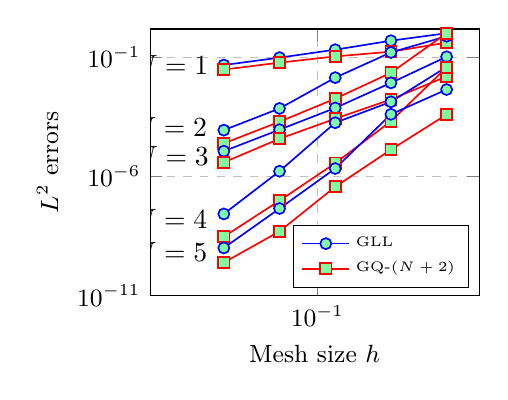
\begin{tikzpicture}
\begin{loglogaxis}[
    width=.475\textwidth,
    xlabel={Mesh size $h$},
    ylabel={$L^2$ errors}, 
    xmin=.0125, xmax=.75,
    ymin=1e-11, ymax=1.5,
    legend pos=south east, legend cell align=left, legend style={font=\tiny},	
    xmajorgrids=true, ymajorgrids=true, grid style=dashed,
    legend entries={GLL,GQ-$(N+2)$}    
]
\pgfplotsset{
cycle list={
{blue, mark=*}, {red, mark=square*}
}
}
%\addlegendimage{no markers,blue}
%\addlegendimage{no markers,red}

\addplot+[semithick, mark options={fill=markercolor}]
% N = 1, tau = 0.000000 =======================
coordinates{(0.5,1)(0.25,0.485059)(0.125,0.203599)(0.0625,0.0947163)(0.03125,0.0463705)};
\addplot+[semithick, mark options={fill=markercolor}]
%N = 1, tau = 0.000000 =======================
coordinates{(0.5,0.402314)(0.25,0.167917)(0.125,0.106574)(0.0625,0.058359)(0.03125,0.0298728)}
[yshift=2pt] node[left, pos=1.025, color=black] {$N = 1$};


\addplot+[semithick, mark options={fill=markercolor}]
% N = 2, tau = 0.000000 =======================
coordinates{(0.5,0.746606)(0.25,0.156701)(0.125,0.0137392)(0.0625,0.000701926)(0.03125,8.64531e-05)};
\addplot+[semithick, mark options={fill=markercolor}]
%N = 2, tau = 0.000000 =======================
coordinates{(0.5,0.993771)(0.25,0.0219437)(0.125,0.00180028)(0.0625,0.000194939)(0.03125,2.4045e-05)}
[yshift=7pt] node[left, pos=1.025, color=black] {$N = 2$};


\addplot+[semithick, mark options={fill=markercolor}]
% N = 3, tau = 0.000000 =======================
coordinates{(0.5,0.103299)(0.25,0.00829887)(0.125,0.00073573)(0.0625,9.05975e-05)(0.03125,1.13596e-05)};
\addplot+[semithick, mark options={fill=markercolor}]
%N = 3, tau = 0.000000 =======================
coordinates{(0.5,0.0154054)(0.25,0.00167426)(0.125,0.000260859)(0.0625,3.76182e-05)(0.03125,3.86238e-06)}
[yshift=3pt] node[left, pos=1.025, color=black] {$N = 3$};

\addplot+[semithick, mark options={fill=markercolor}]
% N = 4, tau = 0.000000 =======================
coordinates{(0.5,0.0385542)(0.25,0.00133048)(0.125,0.000176663)(0.0625,1.64135e-06)(0.03125,2.66024e-08)};
\addplot+[semithick, mark options={fill=markercolor}]
%N = 4, tau = 0.000000 =======================
coordinates{(0.5,0.0367592)(0.25,0.000202817)(0.125,3.57758e-06)(0.0625,9.58294e-08)(0.03125,2.94985e-09)}[yshift=8pt] node[left, pos=1.025, color=black] {$N = 4$};

\addplot+[semithick, mark options={fill=markercolor}]
% N = 5, tau = 0.000000 =======================
coordinates{(0.5,0.00436131)(0.25,0.00039846)(0.125,2.1282e-06)(0.0625,4.49046e-08)(0.03125,9.99912e-10)};
\addplot+[semithick, mark options={fill=markercolor}]
%N = 5, tau = 0.000000 =======================
coordinates{(0.5,0.000390565)(0.25,1.31188e-05)(0.125,3.6544e-07)(0.0625,4.95271e-09)(0.03125,2.42763e-10)}
[yshift=5pt] node[left, pos=1.025, color=black] {$N = 5$};

%\legend{$N=1$,$N=2$,$N=3$,$N=4$,$N=5$}
\end{loglogaxis}
\end{tikzpicture}
}
\subfloat[With Lax-Friedrichs penalization]{
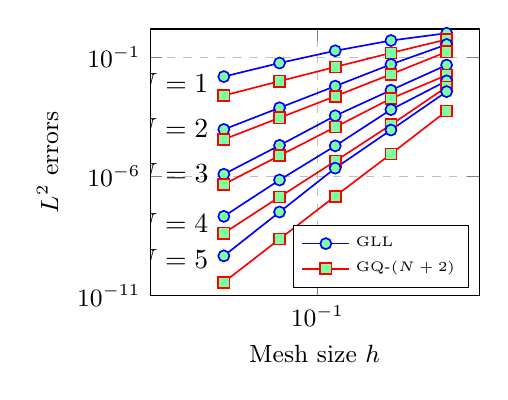
\begin{tikzpicture}
\begin{loglogaxis}[
    width=.475\textwidth,
    xlabel={Mesh size $h$},  ylabel={$L^2$ errors}, 
    xmin=.0125, xmax=.75,
    ymin=1e-11, ymax=1.5,
    legend pos=south east, legend cell align=left, legend style={font=\tiny},	
    xmajorgrids=true, ymajorgrids=true, grid style=dashed,
    legend entries={GLL,GQ-$(N+2)$}
] 
\pgfplotsset{
cycle list={
{blue, mark=*}, {red, mark=square*}
}
}
%\addlegendimage{no markers,blue}
%\addlegendimage{no markers,red}

\addplot+[semithick, mark options={fill=markercolor}]
% N = 1, tau = 0.500000 =======================
coordinates{(0.5,1)(0.25,0.4932)(0.125,0.183839)(0.0625,0.0562398)(0.03125,0.0151873)};
\addplot+[semithick, mark options={fill=markercolor}]
%N = 1, tau = 0.500000 =======================
coordinates{(0.5,0.547558)(0.25,0.148981)(0.125,0.0384647)(0.0625,0.00974763)(0.03125,0.00244539)}
[yshift=5pt] node[left, pos=1.025, color=black] {$N = 1$};

\addplot+[semithick, mark options={fill=markercolor}]	
% N = 2, tau = 0.500000 =======================
coordinates{(0.5,0.336817)(0.25,0.04941)(0.125,0.00605428)(0.0625,0.000748842)(0.03125,9.25456e-05)};
\addplot+[semithick, mark options={fill=markercolor}]
%N = 2, tau = 0.500000 =======================
coordinates{(0.5,0.165807)(0.25,0.0190013)(0.125,0.00227903)(0.0625,0.00028425)(0.03125,3.54865e-05)}
[yshift=5pt] node[left, pos=1.025, color=black] {$N = 2$};


% N = 3, tau = 0.500000 =======================
\addplot+[semithick, mark options={fill=markercolor}]
coordinates{(0.5,0.0463242)(0.25,0.00408748)(0.125,0.000346831)(0.0625,1.99064e-05)(0.03125,1.22357e-06)};
\addplot+[semithick, mark options={fill=markercolor}]
%N = 3, tau = 0.500000 =======================
coordinates{(0.5,0.0174194)(0.25,0.00182234)(0.125,0.000116147)(0.0625,7.39839e-06)(0.03125,4.6305e-07)}
[yshift=5pt] node[left, pos=1.025, color=black] {$N = 3$};

\addplot+[semithick, mark options={fill=markercolor}]
% N = 4, tau = 0.500000 =======================
coordinates{(0.5,0.0100716)(0.25,0.000625923)(0.125,1.89866e-05)(0.0625,7.03865e-07)(0.03125,2.10265e-08)};
\addplot+[semithick, mark options={fill=markercolor}]
%N = 4, tau = 0.500000 =======================
coordinates{(0.5,0.00556743)(0.25,0.000144595)(0.125,4.33972e-06)(0.0625,1.37151e-07)(0.03125,4.16335e-09)}
[yshift=5pt] node[left, pos=1.025, color=black] {$N = 4$};


\addplot+[semithick, mark options={fill=markercolor}]
% N = 5, tau = 0.500000 =======================
coordinates{(0.5,0.00356628)(0.25,8.73125e-05)(0.125,2.20528e-06)(0.0625,3.20127e-08)(0.03125,4.63639e-10)};
\addplot+[semithick, mark options={fill=markercolor}]
%N = 5, tau = 0.500000 =======================
coordinates{(0.5,0.000547621)(0.25,8.7194e-06)(0.125,1.47105e-07)(0.0625,2.34345e-09)(0.03125,3.65306e-11)}
[yshift=10pt] node[left, pos=1.025, color=black] {$N = 5$};

\end{loglogaxis}
\end{tikzpicture}
}
\caption{$L^2$ errors under mesh refinement for entropy conservative and Lax-Friedrichs fluxes under both Gauss-Legendre-Lobatto (GLL) and over-integrated $(N+2)$ point Gauss quadrature (GQ-$(N+2)$).}
\label{fig:convergence}
\end{figure}
We begin by verifying the high order accuracy of the proposed methods using a periodic entropy wave solution
\[
\rho(x,t) = 2 + \sin\LRp{\pi (x - t)}, \qquad u(x,t) = 1, \qquad p(x,t) = 1.
\]
We compute the $L^2$ error in the conservation variables 
\[
\nor{\bm{u} - \bm{u}_h}_{L^2}^2 = \nor{\rho - \rho_h}_{L^2}^2 + \nor{m - m_h}_{L^2}^2 + \nor{E - E_h}_{L^2}^2
\]
at final time $T = .7$ using both the entropy conservative and local Lax-Friedrichs fluxes.  For these experiments, we compare two quadrature rules: the $(N+1)$ point Gauss-Legendre-Lobatto rule (which induces a DG-SEM discretization and is referred to in Figure~\ref{fig:convergence} as ``GLL'') and an $(N+2)$ point Gauss quadrature rule (referred to in the figure as ``GQ-$(N+2)$'').  We do not compare against the $(N+1)$ point Gauss quadrature rule, which behaves very similarly to the GQ-$(N+2)$ case.  The $L^2$ error is evaluated using a more accurate $N+5$ point Gauss quadrature rule, and a CFL of $.125$ is used.  

\begin{table}[h!]
\centering
 \begin{tabular}{||c | c |c |c |c | c|} 
 \hline
 &  $N=1$ &  $N=2$ &  $N=3$ &  $N=4$ &  $N=5$\\
 \hline
 GLL (entropy conservative) & 1.0672 & 3.6561  &  3.0086 &   6.3486 &   5.5278\\ 
 \hline
 GQ-$(N+2)$ (entropy conservative) &  0.9175  &  3.1132  &  3.0388 &   5.1221 &   5.2779 \\ 
 \hline
 GLL (Lax-Friedrichs) & 1.8887  &  3.0164  &  4.0241 &   5.0650 &   6.1095\\ 
 \hline
 GQ-$(N+2)$ (Lax-Friedrichs) & 1.9950  &  3.0018  &  3.9980  &  5.0419  &  6.0034\\ 
 \hline
 \end{tabular}
 \caption{Computed asymptotic convergence rates of $L^2$ errors under mesh refinement.}
 \label{tab:rates}
\end{table}

Figure~\ref{fig:convergence} shows computed $L^2$ errors under mesh refinement for both GLL and GQ-$(N+2)$ quadrature rules.  All experiments utilize the entropy conservative flux of Chandreshekar, and we compare errors with and without Lax-Friedrichs penalization.  Computed asymptotic convergence rates are reported in Table~\ref{tab:rates}.  It can be observed that, for both GLL and GQ-$(N+2)$ quadratures, the entropy conservative flux exhibits suboptimal convergence rates for odd orders, while the inclusion of Lax-Friedrichs penalization restores exhibits the optimal $O(h^{N+1})$ convergence rate for both quadrature choices.

Next, we examine the discrete evolution of entropy by evolving a discontinuous initial profile to final time $T=4$.  We initialize the density and velocity to be 
\begin{equation}
\rho(x,t) = \begin{cases}
3 & \LRb{x} < 1/2\\
2 & \text{otherwise},
\end{cases} \qquad 
u(x,t) = 0, \qquad
p(x,t) = \rho^\gamma.
\label{eq:discontin}
\end{equation}
Non-physical periodic boundary conditions are enforced in order to examine the evolution of entropy over longer time periods.  Figure~\ref{subfig:sol} shows $\rho, u$ at time $T = 1/10$ using both entropy conservative and Lax-Friedrichs fluxes (referred to as ``EC'' and ``LF'', respectively in the figure) and GQ-$(N+2)$ quadrature.  As expected, the entropy conservative flux results in spurious high frequency oscillations, which are significantly damped under Lax-Friedrichs penalization.  

We note that, while the proof of conservation of entropy holds at the semi-discrete level, it does not take into account the time discretization and thus does not hold at the fully discrete level.  This is reflected into numerical observation that the change in entropy $\Delta U(t) = U\LRp{\bm{u}(t}) - U\LRp{\bm{u}(t)}$ increases as $t$ increases.  However, numerical experiments in \cite{gassner2016well} suggest that the discrete change in entropy over time should converge to zero as the timestep decreases, which (under appropriate assumptions) implies that the fully discrete scheme converges to the semi-discrete scheme.  

Figure~\ref{subfig:dS} shows the evolution of $\Delta U(t)$ to final time $T=2$ for both entropy conservative and Lax-Friedrichs fluxes at various CFL numbers.  For the entropy conservative flux, we observe that $\Delta U(t)$ to decreases as the CFL and $\Delta t$ decrease.  This is expected, since the discrete time problem should converge to the continuous semi-discrete problem (for which $\Delta U(t) = 0$) as $\Delta t\rightarrow 0$.  We also observe that, as expected, $\Delta U(t)$ does not change significantly with CFL for the Lax-Friedrichs flux, indicating that the change in entropy is due to the effect of the dissipative flux rather than the time discretization.

\begin{figure}
\centering
\subfloat[Solution at time $T = .1$]{
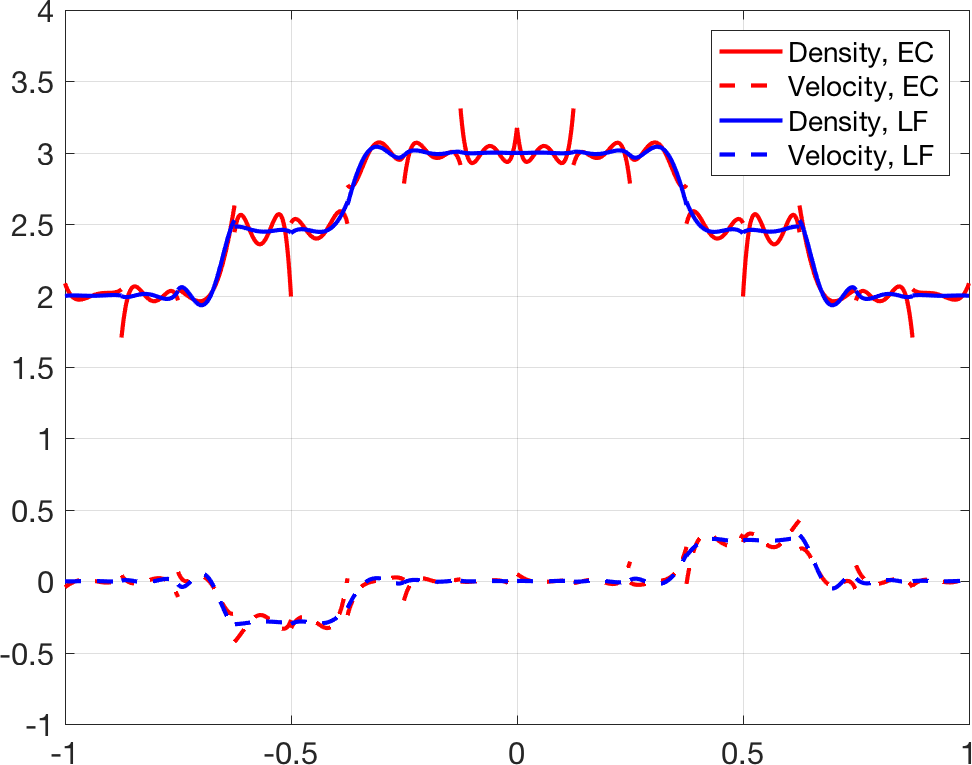
\includegraphics[width=.475\textwidth]{figs/sol_ECLF.png}
\label{subfig:sol}}
\hspace{.5em}
\subfloat[$\Delta U(t)$]{
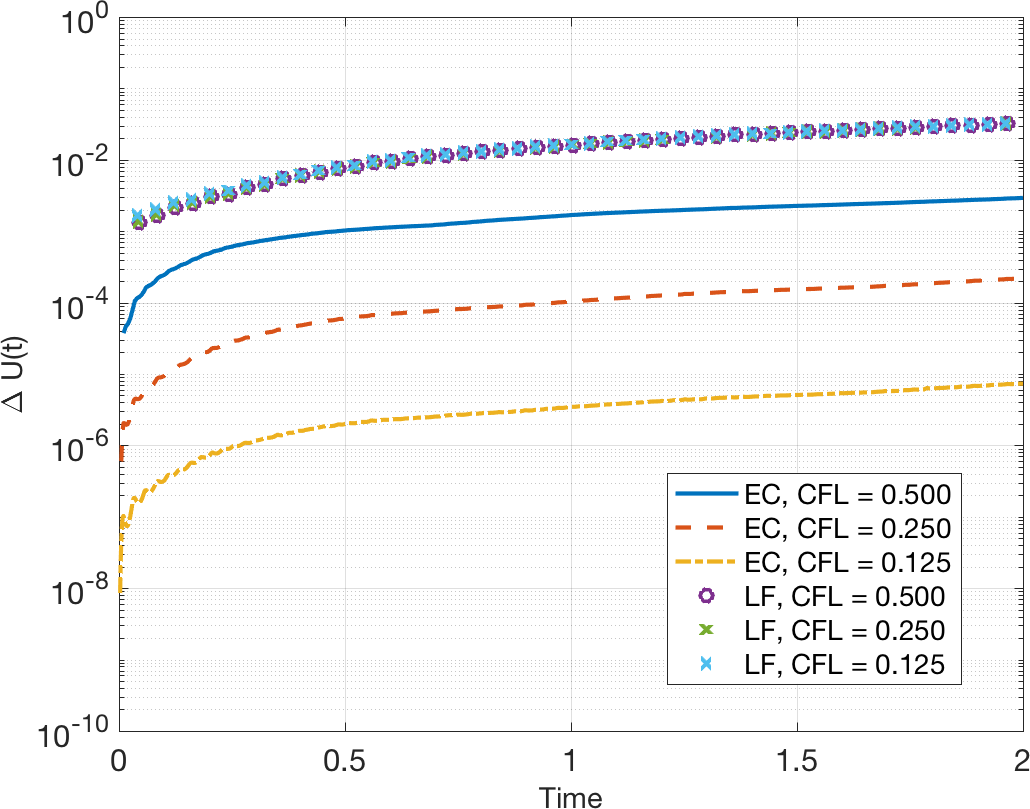
\includegraphics[width=.475\textwidth]{figs/dS_ECLF.png}
\label{subfig:dS}}
\caption{Solution snapshot and change in entropy $\Delta U(t)$ for both entropy conservative (EC) and Lax-Friedrichs (LF) fluxes.}
\label{fig:dS}
\end{figure}

We also numerically evaluate the spatial formulation tested against the projected the entropy variables
\[
\delta(t) = \LRb{\LRp{\left.\LRp{D^x_h \bm{f}_S(\bm{u}_{\bm{v}}(x),\bm{u}_{\bm{v}}(y))}\right|_{y=x},\Pi_N \bm{v}}_{\Omega}}, \qquad  \qquad 0\leq t \leq T.
\]
We utilize the non-dissipative entropy conservative flux and evolve the initial profile (\ref{eq:discontin}) until time $T = 1$ using a GQ-$(N+2)$ quadrature rule.  From Theorem~\ref{thm:ecdg_global}, we expect $\delta_{\max} = \max_{t\in (0,T)}{\delta}$ to be machine zero.  In practice, we have found that $\delta_{\max}$ depends on the tolerance $\epsilon$ used in evaluation of the logarithmic mean.  For a simulation to time $T=4$ using $N=4$ and $K = 16$ with a CFL of $1/2$, we observe that using $\epsilon = 10^{-2}$ (as recommended in \cite{ismail2009affordable} results in $\delta_{\max} = O\LRp{10^{-10}}$.  Decreasing $\epsilon$ to $10^{-3}$ reduces $\delta_{\max}$ to $O\LRp{10^{-14}}$, and decreasing $\epsilon$ further to $1\times 10^{-4}$ reduces $\delta_{\max}$ to $10^{-15}$.  Smaller values of $\epsilon$ do result in observable changes to $\delta_{\max}$, and we do not observe any significant dependence of $\delta_{\max}$ on other discretization parameters.  

\begin{figure}
\centering
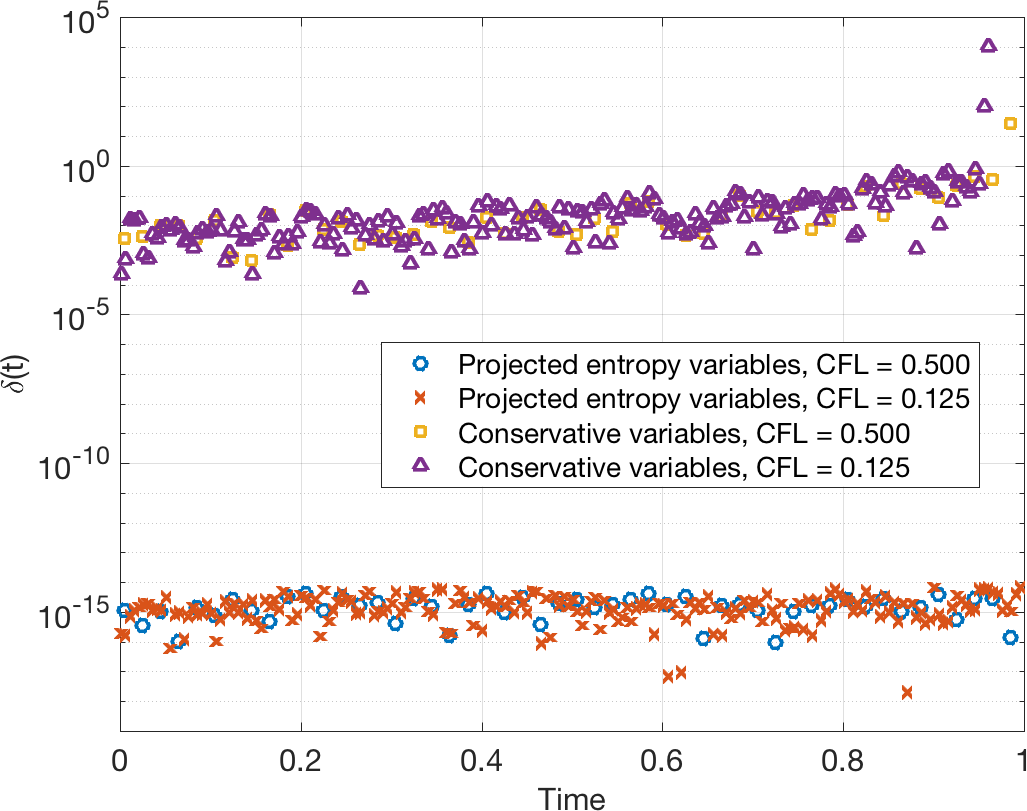
\includegraphics[width=.5\textwidth]{figs/rhstest.png}
\caption{Comparison of $\delta(t)$ when evaluating the flux function $\bm{f}_S$ using conservative variables and projected entropy variables.}
\label{fig:rhstest}
\end{figure}
Finally, in order to illustrate the importance of evaluating the flux in terms of the projected entropy variables $\Pi_N \bm{v}$, we compute $\delta(t)$ while evaluating the flux function $\bm{f}_S$ directly in terms of the conservative variables $\bm{u}(x)$ and in terms of $\bm{u}\LRp{(\Pi_N \bm{v})(x)}$.  It can be observed from Figure~\ref{fig:rhstest} that $\delta(t)$ is near machine precision when evaluating the flux in terms of the projected entropy variables.  When evaluating the flux function using the conservative variables directly, $\delta(t)$ begins near $10^{-4}$ but grows steadily, blowing up exponentially near $t = 1$.  

\section{Conclusions}

This work presents a generalization of discretely entropy conservative methods from diagonal-norm SBP-DG methods to a more general class of high order DG methods which include dense norm SBP methods and over-integrated quadrature rules.  The resulting DG methods satisfy a discrete conservation of entropy while maintaining a reasonable computational cost and small stencil.  Numerical experiments indicate the resulting methods deliver high order accuracy for smooth solutions while displaying greatly improved stability for under-resolved and shock solutions.  

While entropy conservative and stability improve the robustness of solvers for nonlinear hyperbolic conservation laws, they do not address problems such as spurious oscillations in high order approximations of shock solutions or positivity preservation of density and pressure variables \cite{chen2017entropy}.  These issues can be addressed through the use of regularization (e.g.\ filtering, artificial viscosity) and/or limiting; however, the goal in constructing discretely entropy stable methods is to avoid using excessive regularization and limiting in the pursuit of stability.  

Finally, we note that the analysis and numerical experiments in this work are presented in one dimension for clarity and conciseness of presentation.  The main concepts are directly extendable to higher dimensions and simplicial and pyramidal elements, which will be the focus of future work.  

%\note{
%Open question: it's consistent with existing entropy stable collocation DG discretizations, but is the use of $\bm{u}\LRp{\Pi_N \bm{v}}$; is this consistent, can we show this converges?  
%}

\section{Acknowledgments}

The author thanks Andrew Winters, David M.\ Williams, and Paul Hand for informative discussions.  Jesse Chan is supported by NSF awards DMS-1719818 and DMS-1712639.  

\appendix
\section{Assumptions on the flux function}
\label{appendix:A}

In this work, we assume that the flux function $\bm{f}_S$ admits an absolutely convergent expansion of the form
\[
\bm{f}_S(x,y) = \sum_{i=1}^{\infty} \bm{f}_i(x) \bm{g}_i(y), 
\]
where $\bm{f}_i, \bm{g}_i$ are real and bounded over each element $D^k$.  This holds, for example, for analytic $\bm{f}_S$, for which the Taylor series can be rearranged to yield the form of the desired expansion.  This assumption is trivially satisfied for the Burgers' and shallow water equations, as the flux functions consist only of finite sums of products of variables.  However, for the compressible Euler equations, this expansion is less clear due to the presence of the logarithmic mean in the entropy conservative Chandreshekar flux and the presence of inverses of averages and logarithmic means of the variable $\beta = \rho/(2p)$.  

%\note{For Burgers and shallow water, this sum is finite.  
%For the Chandreshekar flux, we consider individual components: the logarithmic mean $L(x,y)$ admits a convergent expansion and is analytic in $x$ \cite{mustonen2002logarithmic}.  CH's flux introduces rational denominators involving the mean and log-mean of $\beta = \rho/(2p)$, which is bounded away from zero if the density and temperature are bounded away from zero.  By composition and products of analytic functions, the CH flux is also analytic. }

We first address the logarithmic mean by noting that it can be expanded out into series form using multi-index notation \cite{mustonen2002logarithmic}.  Let $\mu= (\mu_1,\mu_2)$ be positive integers and define $\LRb{\mu} = \mu_1 + \mu_2$; then, the logarithmic mean can be rewritten as
\[
\frac{x - y}{\log(x)-\log(y)} = \sum_{n=0}^{\infty} \frac{x_n}{n!}, \qquad x_n = \sum_{\LRb{\mu} = n} \frac{\log(x)^{\mu_1}\log(y)^{\mu_2}}{n+1},
\]
where division by $(n+1)$ averages over the $(n+1)$ different permutations of $\mu_1,\mu_2 \geq 0$ which sum to $n$.  
Since $x_n$ is the average of degree $n$ powers of $\log(x),\log(y)$, we have that
\[
%\LRb{x_n} \leq \max{\LRb{\log(x)^n,\log(y)^n}}, \qquad 
\LRb{\frac{x_n}{n!}} \leq \frac{\max{\LRb{\log(x),\log(y)}}^n}{n!}. 
\]
The latter term is simply the $n$th term of the exponential Taylor series evaluated with the argument $\max{\LRb{\log(x),\log(y)}}$.  Because the exponential Taylor series converges absolutely everywhere, the series for the logarithmic mean also converges absolutely for $x,y$ bounded away from $0$ and $\infty$ (i.e.\ $x,y$ are in the logarithmic interval of convergence).  

The entropy conservative Chandreshekar flux also requires multiplication by the terms
\[
\frac{1}{\avg{\beta}}, \qquad \frac{1}{\avg{\beta}^{\log}}, \qquad \beta = \frac{\rho}{2p}.
\]
These terms are analytic if $\avg{\beta}, \avg{\beta}^{\log}$ are bounded away from zero, which is satisfied if the density and pressure are bounded from below as assumed in (\ref{eq:assumption2}).  Because the composition, sum, and product of analytic functions are also analytic, the Chandreshekar flux also is analytic under positivity assumptions.  

Finally, we note that the application of the operator $D_N$ to convergent infinite sums should be rigorously justified.  
This requires $D_N$ to be a bounded operator from $H^1$ to $P^N$, which can be shown using boundedness of the $L^2$ projection operator and discrete inverse and trace inequalities \cite{chan2015gpu}.  

\bibliographystyle{unsrt}
\bibliography{dg}


\end{document}


